% Options for packages loaded elsewhere
\PassOptionsToPackage{unicode}{hyperref}
\PassOptionsToPackage{hyphens}{url}
%
\documentclass[
]{article}
\usepackage{amsmath,amssymb}
\usepackage{lmodern}
\usepackage{ifxetex,ifluatex}
\ifnum 0\ifxetex 1\fi\ifluatex 1\fi=0 % if pdftex
  \usepackage[T1]{fontenc}
  \usepackage[utf8]{inputenc}
  \usepackage{textcomp} % provide euro and other symbols
\else % if luatex or xetex
  \usepackage{unicode-math}
  \defaultfontfeatures{Scale=MatchLowercase}
  \defaultfontfeatures[\rmfamily]{Ligatures=TeX,Scale=1}
\fi
% Use upquote if available, for straight quotes in verbatim environments
\IfFileExists{upquote.sty}{\usepackage{upquote}}{}
\IfFileExists{microtype.sty}{% use microtype if available
  \usepackage[]{microtype}
  \UseMicrotypeSet[protrusion]{basicmath} % disable protrusion for tt fonts
}{}
\makeatletter
\@ifundefined{KOMAClassName}{% if non-KOMA class
  \IfFileExists{parskip.sty}{%
    \usepackage{parskip}
  }{% else
    \setlength{\parindent}{0pt}
    \setlength{\parskip}{6pt plus 2pt minus 1pt}}
}{% if KOMA class
  \KOMAoptions{parskip=half}}
\makeatother
\usepackage{xcolor}
\IfFileExists{xurl.sty}{\usepackage{xurl}}{} % add URL line breaks if available
\IfFileExists{bookmark.sty}{\usepackage{bookmark}}{\usepackage{hyperref}}
\hypersetup{
  pdftitle={Assignment Journal},
  hidelinks,
  pdfcreator={LaTeX via pandoc}}
\urlstyle{same} % disable monospaced font for URLs
\usepackage[margin=1in]{geometry}
\usepackage{color}
\usepackage{fancyvrb}
\newcommand{\VerbBar}{|}
\newcommand{\VERB}{\Verb[commandchars=\\\{\}]}
\DefineVerbatimEnvironment{Highlighting}{Verbatim}{commandchars=\\\{\}}
% Add ',fontsize=\small' for more characters per line
\usepackage{framed}
\definecolor{shadecolor}{RGB}{248,248,248}
\newenvironment{Shaded}{\begin{snugshade}}{\end{snugshade}}
\newcommand{\AlertTok}[1]{\textcolor[rgb]{0.94,0.16,0.16}{#1}}
\newcommand{\AnnotationTok}[1]{\textcolor[rgb]{0.56,0.35,0.01}{\textbf{\textit{#1}}}}
\newcommand{\AttributeTok}[1]{\textcolor[rgb]{0.77,0.63,0.00}{#1}}
\newcommand{\BaseNTok}[1]{\textcolor[rgb]{0.00,0.00,0.81}{#1}}
\newcommand{\BuiltInTok}[1]{#1}
\newcommand{\CharTok}[1]{\textcolor[rgb]{0.31,0.60,0.02}{#1}}
\newcommand{\CommentTok}[1]{\textcolor[rgb]{0.56,0.35,0.01}{\textit{#1}}}
\newcommand{\CommentVarTok}[1]{\textcolor[rgb]{0.56,0.35,0.01}{\textbf{\textit{#1}}}}
\newcommand{\ConstantTok}[1]{\textcolor[rgb]{0.00,0.00,0.00}{#1}}
\newcommand{\ControlFlowTok}[1]{\textcolor[rgb]{0.13,0.29,0.53}{\textbf{#1}}}
\newcommand{\DataTypeTok}[1]{\textcolor[rgb]{0.13,0.29,0.53}{#1}}
\newcommand{\DecValTok}[1]{\textcolor[rgb]{0.00,0.00,0.81}{#1}}
\newcommand{\DocumentationTok}[1]{\textcolor[rgb]{0.56,0.35,0.01}{\textbf{\textit{#1}}}}
\newcommand{\ErrorTok}[1]{\textcolor[rgb]{0.64,0.00,0.00}{\textbf{#1}}}
\newcommand{\ExtensionTok}[1]{#1}
\newcommand{\FloatTok}[1]{\textcolor[rgb]{0.00,0.00,0.81}{#1}}
\newcommand{\FunctionTok}[1]{\textcolor[rgb]{0.00,0.00,0.00}{#1}}
\newcommand{\ImportTok}[1]{#1}
\newcommand{\InformationTok}[1]{\textcolor[rgb]{0.56,0.35,0.01}{\textbf{\textit{#1}}}}
\newcommand{\KeywordTok}[1]{\textcolor[rgb]{0.13,0.29,0.53}{\textbf{#1}}}
\newcommand{\NormalTok}[1]{#1}
\newcommand{\OperatorTok}[1]{\textcolor[rgb]{0.81,0.36,0.00}{\textbf{#1}}}
\newcommand{\OtherTok}[1]{\textcolor[rgb]{0.56,0.35,0.01}{#1}}
\newcommand{\PreprocessorTok}[1]{\textcolor[rgb]{0.56,0.35,0.01}{\textit{#1}}}
\newcommand{\RegionMarkerTok}[1]{#1}
\newcommand{\SpecialCharTok}[1]{\textcolor[rgb]{0.00,0.00,0.00}{#1}}
\newcommand{\SpecialStringTok}[1]{\textcolor[rgb]{0.31,0.60,0.02}{#1}}
\newcommand{\StringTok}[1]{\textcolor[rgb]{0.31,0.60,0.02}{#1}}
\newcommand{\VariableTok}[1]{\textcolor[rgb]{0.00,0.00,0.00}{#1}}
\newcommand{\VerbatimStringTok}[1]{\textcolor[rgb]{0.31,0.60,0.02}{#1}}
\newcommand{\WarningTok}[1]{\textcolor[rgb]{0.56,0.35,0.01}{\textbf{\textit{#1}}}}
\usepackage{graphicx}
\makeatletter
\def\maxwidth{\ifdim\Gin@nat@width>\linewidth\linewidth\else\Gin@nat@width\fi}
\def\maxheight{\ifdim\Gin@nat@height>\textheight\textheight\else\Gin@nat@height\fi}
\makeatother
% Scale images if necessary, so that they will not overflow the page
% margins by default, and it is still possible to overwrite the defaults
% using explicit options in \includegraphics[width, height, ...]{}
\setkeys{Gin}{width=\maxwidth,height=\maxheight,keepaspectratio}
% Set default figure placement to htbp
\makeatletter
\def\fps@figure{htbp}
\makeatother
\setlength{\emergencystretch}{3em} % prevent overfull lines
\providecommand{\tightlist}{%
  \setlength{\itemsep}{0pt}\setlength{\parskip}{0pt}}
\setcounter{secnumdepth}{-\maxdimen} % remove section numbering
\ifluatex
  \usepackage{selnolig}  % disable illegal ligatures
\fi

\title{Assignment Journal}
\author{}
\date{\vspace{-2.5em}}

\begin{document}
\maketitle

{
\setcounter{tocdepth}{1}
\tableofcontents
}
This is where all of my assignments and exams for CRIM250 are located.

\hypertarget{assignment-1}{%
\section{Assignment 1}\label{assignment-1}}

\hypertarget{problem-1}{%
\subsubsection{Problem 1}\label{problem-1}}

Install the datasets package on the console below using
\texttt{install.packages("datasets")}. Now load the library.

\begin{Shaded}
\begin{Highlighting}[]
\NormalTok{USArrests}
\end{Highlighting}
\end{Shaded}

\begin{verbatim}
##                Murder Assault UrbanPop Rape
## Alabama          13.2     236       58 21.2
## Alaska           10.0     263       48 44.5
## Arizona           8.1     294       80 31.0
## Arkansas          8.8     190       50 19.5
## California        9.0     276       91 40.6
## Colorado          7.9     204       78 38.7
## Connecticut       3.3     110       77 11.1
## Delaware          5.9     238       72 15.8
## Florida          15.4     335       80 31.9
## Georgia          17.4     211       60 25.8
## Hawaii            5.3      46       83 20.2
## Idaho             2.6     120       54 14.2
## Illinois         10.4     249       83 24.0
## Indiana           7.2     113       65 21.0
## Iowa              2.2      56       57 11.3
## Kansas            6.0     115       66 18.0
## Kentucky          9.7     109       52 16.3
## Louisiana        15.4     249       66 22.2
## Maine             2.1      83       51  7.8
## Maryland         11.3     300       67 27.8
## Massachusetts     4.4     149       85 16.3
## Michigan         12.1     255       74 35.1
## Minnesota         2.7      72       66 14.9
## Mississippi      16.1     259       44 17.1
## Missouri          9.0     178       70 28.2
## Montana           6.0     109       53 16.4
## Nebraska          4.3     102       62 16.5
## Nevada           12.2     252       81 46.0
## New Hampshire     2.1      57       56  9.5
## New Jersey        7.4     159       89 18.8
## New Mexico       11.4     285       70 32.1
## New York         11.1     254       86 26.1
## North Carolina   13.0     337       45 16.1
## North Dakota      0.8      45       44  7.3
## Ohio              7.3     120       75 21.4
## Oklahoma          6.6     151       68 20.0
## Oregon            4.9     159       67 29.3
## Pennsylvania      6.3     106       72 14.9
## Rhode Island      3.4     174       87  8.3
## South Carolina   14.4     279       48 22.5
## South Dakota      3.8      86       45 12.8
## Tennessee        13.2     188       59 26.9
## Texas            12.7     201       80 25.5
## Utah              3.2     120       80 22.9
## Vermont           2.2      48       32 11.2
## Virginia          8.5     156       63 20.7
## Washington        4.0     145       73 26.2
## West Virginia     5.7      81       39  9.3
## Wisconsin         2.6      53       66 10.8
## Wyoming           6.8     161       60 15.6
\end{verbatim}

Load the USArrests dataset and rename it \texttt{dat}. Note that this
dataset comes with R, in the package datasets, so there's no need to
load data from your computer. Why is it useful to rename the dataset?

\begin{Shaded}
\begin{Highlighting}[]
\NormalTok{dat}\OtherTok{\textless{}{-}}\NormalTok{USArrests}
\NormalTok{dat.USArrests }\OtherTok{\textless{}{-}}\NormalTok{ dat}
\end{Highlighting}
\end{Shaded}

\emph{Answer:} It is useful to rename the dataset for two reasons.
First, it will help you keep track of your work and not confuse it with
other generic-looking names of other datasets. Second, it will allow you
to keep an original copy of the file while creating a new file with all
of the changes you are currently making on it.

\hypertarget{problem-2}{%
\subsubsection{Problem 2}\label{problem-2}}

Use this command to make the state names into a new variable called
State.

\begin{Shaded}
\begin{Highlighting}[]
\NormalTok{dat.USArrests}\SpecialCharTok{$}\NormalTok{state }\OtherTok{\textless{}{-}} \FunctionTok{tolower}\NormalTok{(}\FunctionTok{rownames}\NormalTok{(USArrests))}
\NormalTok{dat.USArrests}
\end{Highlighting}
\end{Shaded}

\begin{verbatim}
##                Murder Assault UrbanPop Rape          state
## Alabama          13.2     236       58 21.2        alabama
## Alaska           10.0     263       48 44.5         alaska
## Arizona           8.1     294       80 31.0        arizona
## Arkansas          8.8     190       50 19.5       arkansas
## California        9.0     276       91 40.6     california
## Colorado          7.9     204       78 38.7       colorado
## Connecticut       3.3     110       77 11.1    connecticut
## Delaware          5.9     238       72 15.8       delaware
## Florida          15.4     335       80 31.9        florida
## Georgia          17.4     211       60 25.8        georgia
## Hawaii            5.3      46       83 20.2         hawaii
## Idaho             2.6     120       54 14.2          idaho
## Illinois         10.4     249       83 24.0       illinois
## Indiana           7.2     113       65 21.0        indiana
## Iowa              2.2      56       57 11.3           iowa
## Kansas            6.0     115       66 18.0         kansas
## Kentucky          9.7     109       52 16.3       kentucky
## Louisiana        15.4     249       66 22.2      louisiana
## Maine             2.1      83       51  7.8          maine
## Maryland         11.3     300       67 27.8       maryland
## Massachusetts     4.4     149       85 16.3  massachusetts
## Michigan         12.1     255       74 35.1       michigan
## Minnesota         2.7      72       66 14.9      minnesota
## Mississippi      16.1     259       44 17.1    mississippi
## Missouri          9.0     178       70 28.2       missouri
## Montana           6.0     109       53 16.4        montana
## Nebraska          4.3     102       62 16.5       nebraska
## Nevada           12.2     252       81 46.0         nevada
## New Hampshire     2.1      57       56  9.5  new hampshire
## New Jersey        7.4     159       89 18.8     new jersey
## New Mexico       11.4     285       70 32.1     new mexico
## New York         11.1     254       86 26.1       new york
## North Carolina   13.0     337       45 16.1 north carolina
## North Dakota      0.8      45       44  7.3   north dakota
## Ohio              7.3     120       75 21.4           ohio
## Oklahoma          6.6     151       68 20.0       oklahoma
## Oregon            4.9     159       67 29.3         oregon
## Pennsylvania      6.3     106       72 14.9   pennsylvania
## Rhode Island      3.4     174       87  8.3   rhode island
## South Carolina   14.4     279       48 22.5 south carolina
## South Dakota      3.8      86       45 12.8   south dakota
## Tennessee        13.2     188       59 26.9      tennessee
## Texas            12.7     201       80 25.5          texas
## Utah              3.2     120       80 22.9           utah
## Vermont           2.2      48       32 11.2        vermont
## Virginia          8.5     156       63 20.7       virginia
## Washington        4.0     145       73 26.2     washington
## West Virginia     5.7      81       39  9.3  west virginia
## Wisconsin         2.6      53       66 10.8      wisconsin
## Wyoming           6.8     161       60 15.6        wyoming
\end{verbatim}

This dataset has the state names as row names, so we just want to make
them into a new variable. We also make them all lower case, because that
will help us draw a map later - the map function requires the states to
be lower case.

List the variables contained in the dataset \texttt{USArrests}.

\begin{Shaded}
\begin{Highlighting}[]
\FunctionTok{names}\NormalTok{(dat.USArrests)}
\end{Highlighting}
\end{Shaded}

\begin{verbatim}
## [1] "Murder"   "Assault"  "UrbanPop" "Rape"     "state"
\end{verbatim}

\emph{Answer:} The variables include Murder, Assault, Rape, Urban
Population, and State.

\hypertarget{problem-3}{%
\subsubsection{Problem 3}\label{problem-3}}

What type of variable (from the DVB chapter) is \texttt{Murder}?

\emph{Answer:} In the DVB chapter, ``Murder'' would be considered a
qualitative, or categorical, variable.

What R Type of variable is it?

\emph{Answer:} ``Murder'' is considered a character in R.

\hypertarget{problem-4}{%
\subsubsection{Problem 4}\label{problem-4}}

What information is contained in this dataset, in general? What do the
numbers mean?

\emph{Answer:} The dataset includes the arrest rates for murder,
assault, and rape per 100,000 residents in each of the US's 50 states.
Additionally, the percent of the population living in urban areas is
given. Here, then, the numbers mean either the arrest rates for a crime
per 100k residents in a state or the percent of residents living in
urban spaces in a state.

\hypertarget{problem-5}{%
\subsubsection{Problem 5}\label{problem-5}}

Draw a histogram of \texttt{Murder} with proper labels and title.

\begin{Shaded}
\begin{Highlighting}[]
\FunctionTok{hist}\NormalTok{(dat.USArrests}\SpecialCharTok{$}\NormalTok{Murder, }\AttributeTok{main=}\StringTok{"Histogram of Murder Rates"}\NormalTok{, }\AttributeTok{xlab=}\StringTok{"Murder Rates per State"}\NormalTok{, }\AttributeTok{ylab=}\StringTok{"Frequency"}\NormalTok{)}
\end{Highlighting}
\end{Shaded}

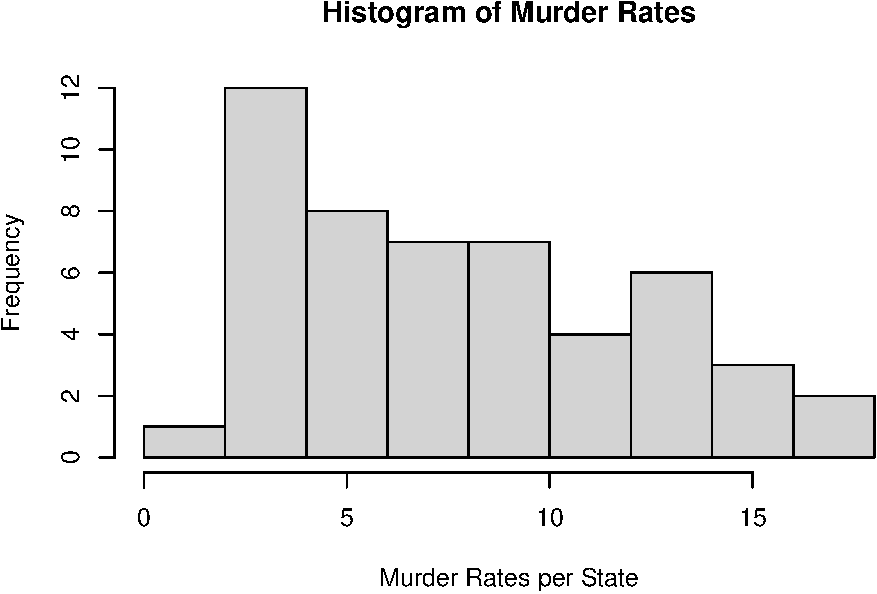
\includegraphics{Journal_files/figure-latex/unnamed-chunk-5-1.pdf}

\hypertarget{problem-6}{%
\subsubsection{Problem 6}\label{problem-6}}

Please summarize \texttt{Murder} quantitatively. What are its mean and
median? What is the difference between mean and median? What is a
quartile, and why do you think R gives you the 1st Qu. and 3rd Qu.?

\begin{Shaded}
\begin{Highlighting}[]
\FunctionTok{summary}\NormalTok{(dat.USArrests}\SpecialCharTok{$}\NormalTok{Murder)}
\end{Highlighting}
\end{Shaded}

\begin{verbatim}
##    Min. 1st Qu.  Median    Mean 3rd Qu.    Max. 
##   0.800   4.075   7.250   7.788  11.250  17.400
\end{verbatim}

\emph{Answer:} The mean of ``Murder'' is 7.788, while its median is
7.250. Generally, mean signifies the solution of all of the values added
together and then divided by the number of values, while median
signifies the middle value when all values are lined up in ascending
order. A quartile constitutes one of three values that divides a data
distribution into fourths. Lastly, R would provide the first and third
quartile in order to help the statistician understand where the majority
of values lie (in between the first and third quartile) or what values
might be considered outliers (before the first and after the third).

\hypertarget{problem-7}{%
\subsubsection{Problem 7}\label{problem-7}}

Repeat the same steps you followed for \texttt{Murder}, for the
variables \texttt{Assault} and \texttt{Rape}. Now plot all three
histograms together. You can do this by using the command
\texttt{par(mfrow=c(3,1))} and then plotting each of the three.

\begin{Shaded}
\begin{Highlighting}[]
\FunctionTok{hist}\NormalTok{(dat.USArrests}\SpecialCharTok{$}\NormalTok{Assault, }\AttributeTok{main=}\StringTok{"Histogram of Assault Rates"}\NormalTok{, }\AttributeTok{xlab=}\StringTok{"Assault Rates per State"}\NormalTok{, }\AttributeTok{ylab=}\StringTok{"Frequency"}\NormalTok{)}
\end{Highlighting}
\end{Shaded}

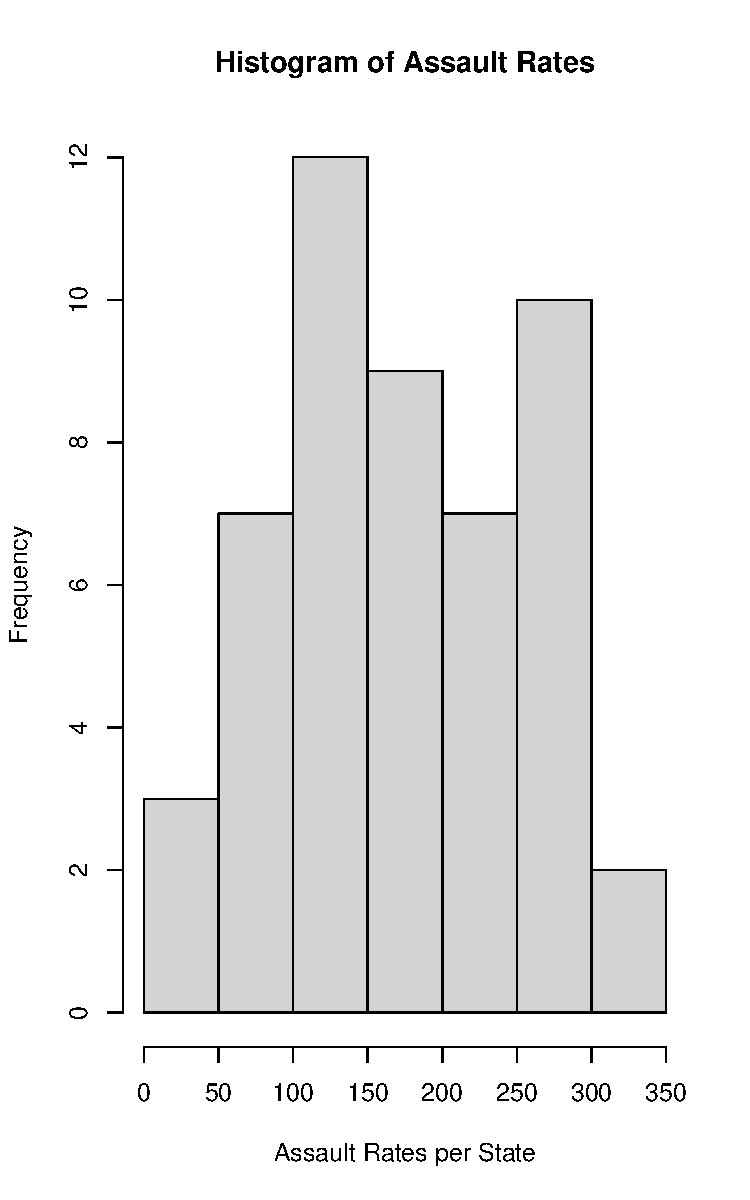
\includegraphics{Journal_files/figure-latex/unnamed-chunk-7-1.pdf}

\begin{Shaded}
\begin{Highlighting}[]
\FunctionTok{hist}\NormalTok{(dat.USArrests}\SpecialCharTok{$}\NormalTok{Rape, }\AttributeTok{main=}\StringTok{"Histogram of Rape Rates"}\NormalTok{, }\AttributeTok{xlab=}\StringTok{"Rape Rates per State"}\NormalTok{, }\AttributeTok{ylab=}\StringTok{"Frequency"}\NormalTok{)}
\end{Highlighting}
\end{Shaded}

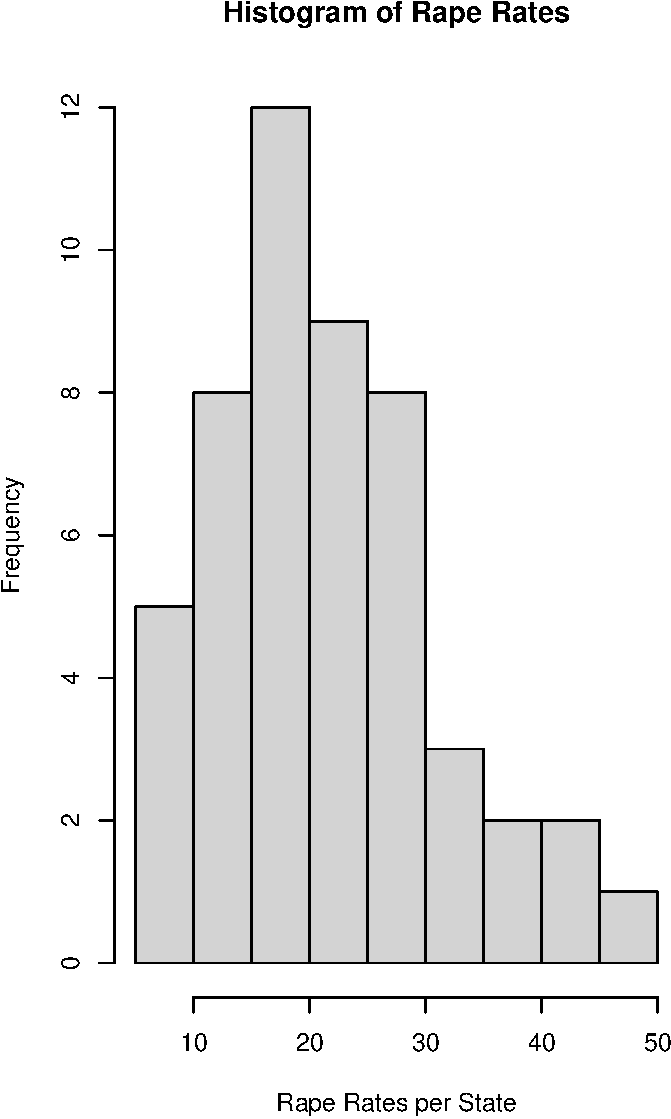
\includegraphics{Journal_files/figure-latex/unnamed-chunk-7-2.pdf}

\begin{Shaded}
\begin{Highlighting}[]
\FunctionTok{par}\NormalTok{(}\AttributeTok{mfrow=}\FunctionTok{c}\NormalTok{(}\DecValTok{3}\NormalTok{,}\DecValTok{1}\NormalTok{))}
\FunctionTok{hist}\NormalTok{(dat.USArrests}\SpecialCharTok{$}\NormalTok{Murder, }\AttributeTok{main=}\StringTok{"Histogram of Murder Rates"}\NormalTok{, }\AttributeTok{xlab=}\StringTok{"Murder Rates per State"}\NormalTok{, }\AttributeTok{ylab=}\StringTok{"Frequency"}\NormalTok{)}
\FunctionTok{hist}\NormalTok{(dat.USArrests}\SpecialCharTok{$}\NormalTok{Assault, }\AttributeTok{main=}\StringTok{"Histogram of Assault Rates"}\NormalTok{, }\AttributeTok{xlab=}\StringTok{"Assault Rates per State"}\NormalTok{, }\AttributeTok{ylab=}\StringTok{"Frequency"}\NormalTok{)}
\FunctionTok{hist}\NormalTok{(dat.USArrests}\SpecialCharTok{$}\NormalTok{Rape, }\AttributeTok{main=}\StringTok{"Histogram of Rape Rates"}\NormalTok{, }\AttributeTok{xlab=}\StringTok{"Rape Rates per State"}\NormalTok{, }\AttributeTok{ylab=}\StringTok{"Frequency"}\NormalTok{)}
\end{Highlighting}
\end{Shaded}

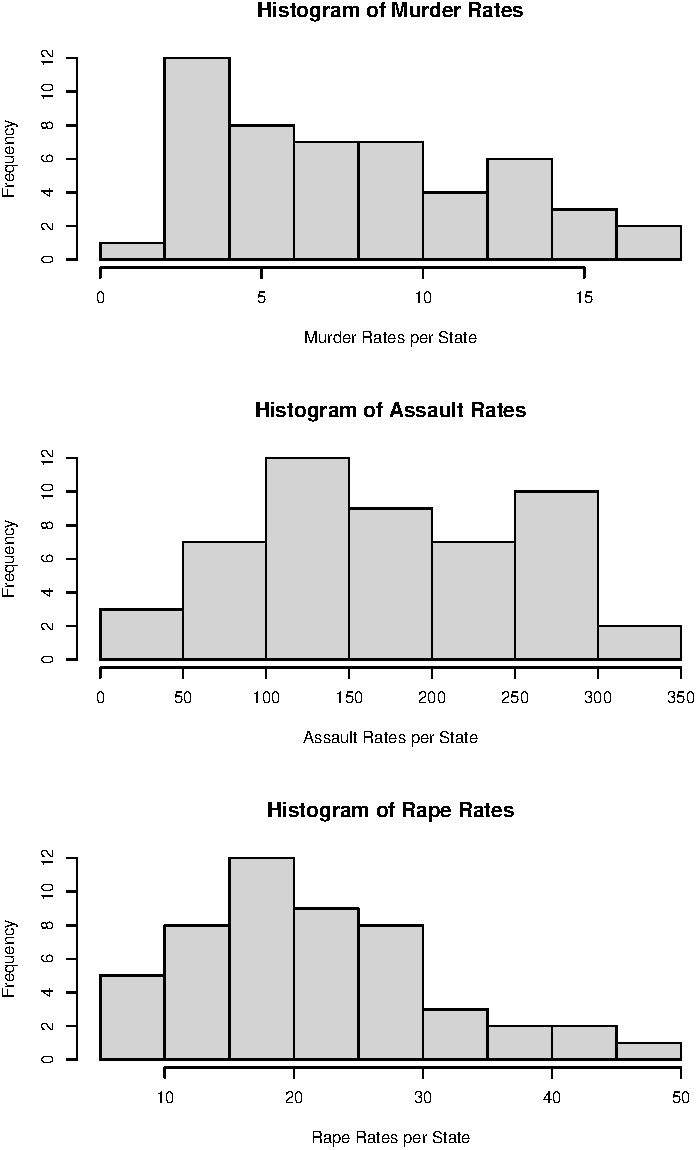
\includegraphics{Journal_files/figure-latex/unnamed-chunk-8-1.pdf}

What does the command par do, in your own words (you can look this up by
asking R \texttt{?par})?

\emph{Answer:} The command par enables the statistician to set graphical
parameters for data in either a singular graph or multiple graphs.

What can you learn from plotting the histograms together?

\emph{Answer:} By plotting histograms together, you are able to compare
the data between different categories -- in this case, comparing the
differences in assault and murder rates per state, for example.
Additionally, you can gain a better understand of the data overall by
looking at it holistically instead of piece-by-piece.

\hypertarget{problem-8}{%
\subsubsection{Problem 8}\label{problem-8}}

In the console below (not in text), type
\texttt{install.packages("maps")} and press Enter, and then type
\texttt{install.packages("ggplot2")} and press Enter. This will install
the packages so you can load the libraries.

Run this code:

\begin{Shaded}
\begin{Highlighting}[]
\FunctionTok{library}\NormalTok{(}\StringTok{\textquotesingle{}maps\textquotesingle{}}\NormalTok{) }
\FunctionTok{library}\NormalTok{(}\StringTok{\textquotesingle{}ggplot2\textquotesingle{}}\NormalTok{) }

\FunctionTok{ggplot}\NormalTok{(dat, }\FunctionTok{aes}\NormalTok{(}\AttributeTok{map\_id=}\NormalTok{state, }\AttributeTok{fill=}\NormalTok{Murder)) }\SpecialCharTok{+} 
  \FunctionTok{geom\_map}\NormalTok{(}\AttributeTok{map=}\FunctionTok{map\_data}\NormalTok{(}\StringTok{"state"}\NormalTok{)) }\SpecialCharTok{+} 
  \FunctionTok{expand\_limits}\NormalTok{(}\AttributeTok{x=}\FunctionTok{map\_data}\NormalTok{(}\StringTok{"state"}\NormalTok{)}\SpecialCharTok{$}\NormalTok{long, }\AttributeTok{y=}\FunctionTok{map\_data}\NormalTok{(}\StringTok{"state"}\NormalTok{)}\SpecialCharTok{$}\NormalTok{lat)}
\end{Highlighting}
\end{Shaded}

What does this code do? Explain what each line is doing.

\emph{Answer:} This code is mapping the arrest rates of murder per
100,000 citizens per state. With this, we are able to see the salience
and prominence of arrest rates through a colored map of the United
States. The first line is using the data groups of ``state'' and
``Murder'' to construct aesthetic mapping in a ggplot, filling the map
with ``Murder'' rates. Next, the second line is the direction to map the
states, while the third line is expanding the x and y axes,
i.e.~longitude and latitude, in the graph.

\hypertarget{assignment-2}{%
\section{Assignment 2}\label{assignment-2}}

\hypertarget{problem-1-load-data}{%
\subsubsection{Problem 1: Load Data}\label{problem-1-load-data}}

\begin{Shaded}
\begin{Highlighting}[]
\NormalTok{dat }\OtherTok{\textless{}{-}} \FunctionTok{read.csv}\NormalTok{(}\AttributeTok{file =} \StringTok{\textquotesingle{}dat.nsduh.small.1.csv\textquotesingle{}}\NormalTok{)}
\FunctionTok{head}\NormalTok{(dat)}
\end{Highlighting}
\end{Shaded}

\begin{verbatim}
##   mjage cigage iralcage age2 sexatract speakengl irsex
## 1    14     50       14   16         1         1     1
## 2    11     14        5   13         2         1     2
## 3    12     35       12   15         2         1     2
## 4    16     18       18   14         1         1     1
## 5    14     16       14   16         4         1     1
## 6    12     16       18   15         4         1     2
\end{verbatim}

\emph{What are the dimensions of the data set?}

\begin{Shaded}
\begin{Highlighting}[]
\FunctionTok{names}\NormalTok{(dat)}
\end{Highlighting}
\end{Shaded}

\begin{verbatim}
## [1] "mjage"     "cigage"    "iralcage"  "age2"      "sexatract" "speakengl"
## [7] "irsex"
\end{verbatim}

\hypertarget{problem-2-variables}{%
\subsubsection{Problem 2: Variables}\label{problem-2-variables}}

\emph{Describe the variables in the dataset}

The variables are forms of quantitative variables, and all the datasets
are described as integers within R. Here, these variables are labeled as
mjage (age of first use of marijuana), cigage (age of first daily use of
cigarettes), iralcage (age that first tried alcohol), age2 (age recorded
the second time), sexatract (sexual attraction/action towards different
genders), speakengl (proficiency in English), and irsex (sex of
individual).

\begin{Shaded}
\begin{Highlighting}[]
\FunctionTok{class}\NormalTok{(dat}\SpecialCharTok{$}\NormalTok{mjage)}
\end{Highlighting}
\end{Shaded}

\begin{verbatim}
## [1] "integer"
\end{verbatim}

\begin{Shaded}
\begin{Highlighting}[]
\FunctionTok{class}\NormalTok{(dat}\SpecialCharTok{$}\NormalTok{cigage)}
\end{Highlighting}
\end{Shaded}

\begin{verbatim}
## [1] "integer"
\end{verbatim}

\begin{Shaded}
\begin{Highlighting}[]
\FunctionTok{class}\NormalTok{(dat}\SpecialCharTok{$}\NormalTok{iralcage)}
\end{Highlighting}
\end{Shaded}

\begin{verbatim}
## [1] "integer"
\end{verbatim}

\begin{Shaded}
\begin{Highlighting}[]
\FunctionTok{class}\NormalTok{(dat}\SpecialCharTok{$}\NormalTok{age2)}
\end{Highlighting}
\end{Shaded}

\begin{verbatim}
## [1] "integer"
\end{verbatim}

\begin{Shaded}
\begin{Highlighting}[]
\FunctionTok{class}\NormalTok{(dat}\SpecialCharTok{$}\NormalTok{sexatract)}
\end{Highlighting}
\end{Shaded}

\begin{verbatim}
## [1] "integer"
\end{verbatim}

\begin{Shaded}
\begin{Highlighting}[]
\FunctionTok{class}\NormalTok{(dat}\SpecialCharTok{$}\NormalTok{speakengl)}
\end{Highlighting}
\end{Shaded}

\begin{verbatim}
## [1] "integer"
\end{verbatim}

\begin{Shaded}
\begin{Highlighting}[]
\FunctionTok{class}\NormalTok{(dat}\SpecialCharTok{$}\NormalTok{irsex)}
\end{Highlighting}
\end{Shaded}

\begin{verbatim}
## [1] "integer"
\end{verbatim}

\emph{What is this dataset about? Who collected the data, what kind of
sample is it, and what was the purpose of generating the data?}

The data describe a respondent's first use of a variety of substances,
including alcohol, marijuana, and cigarettes, as well as describing the
age, language, sex, and sexual orientation of the respondents. The data
presented in this set are a small sample from the entirety of data
collected by the National Survey of Drug Use and Health. Here, only the
first 1,000 responses are used out of the entire representative sample
taken by the NSDUH. By generating this data, the NSDUH is able to
greater understand the use of particular substances around the country,
as well as the sexual tendencies of individuals, based on age, gender,
and language proficiency.

\hypertarget{problem-3-age-and-gender}{%
\subsubsection{Problem 3: Age and
gender}\label{problem-3-age-and-gender}}

\emph{What is the age distribution of the sample like? Make sure you
read the codebook to know what the variable values mean.}

\begin{Shaded}
\begin{Highlighting}[]
\FunctionTok{hist}\NormalTok{(dat}\SpecialCharTok{$}\NormalTok{age2, }\AttributeTok{main=}\StringTok{"Age of Respondents"}\NormalTok{, }\AttributeTok{xlab =} \StringTok{"Code for Age Group"}\NormalTok{, }\AttributeTok{ylab =} \StringTok{"Frequency"}\NormalTok{)}
\end{Highlighting}
\end{Shaded}

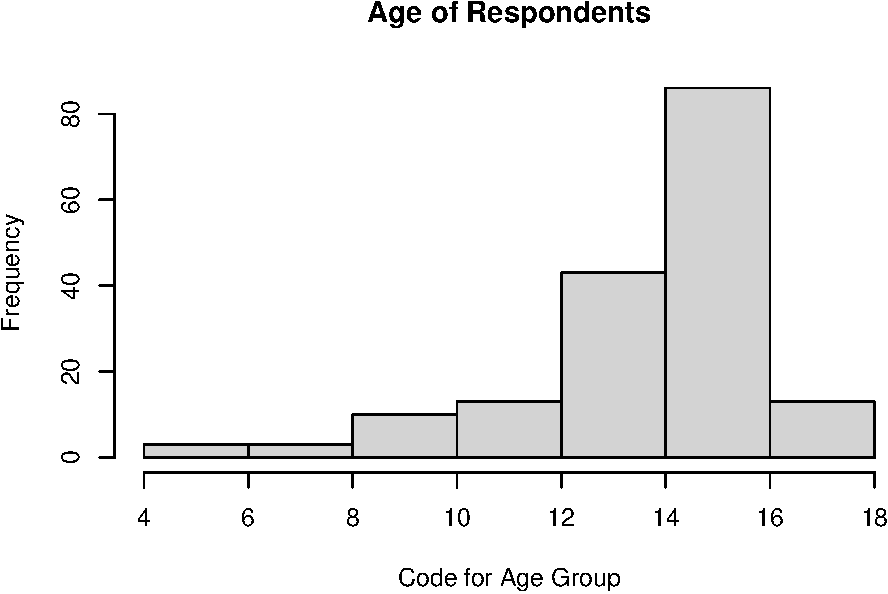
\includegraphics{Journal_files/figure-latex/unnamed-chunk-13-1.pdf}

\emph{Do you think this age distribution representative of the US
population? Why or why not?}

I do not believe this distribution is representative of the US
population, because, more than anything, the way the ages are
distributed in these coded groups are completely skewed, with codes 1-12
solely for individuals at or under 25 years of age, while the codes
12-17 are responsible for the rest of the population's ages. Here,
nearly 2/3 of the codes account for solely over 1/3 of the United States
population (that under 25 years of age). In this data set, there are no
patterns to age distribution, with some codes representing one age,
others representing four, and others representing fourteen.

\emph{Is the sample balanced in terms of gender? If not, are there more
females or males?}

\begin{Shaded}
\begin{Highlighting}[]
\NormalTok{counts }\OtherTok{\textless{}{-}} \FunctionTok{table}\NormalTok{(dat}\SpecialCharTok{$}\NormalTok{irsex)}
\NormalTok{counts}
\end{Highlighting}
\end{Shaded}

\begin{verbatim}
## 
##  1  2 
## 91 80
\end{verbatim}

\begin{Shaded}
\begin{Highlighting}[]
\FunctionTok{barplot}\NormalTok{(counts, }\AttributeTok{main=}\StringTok{"Gender Distribution"}\NormalTok{, }\AttributeTok{xlab=}\StringTok{"Gender"}\NormalTok{, }\AttributeTok{names=}\FunctionTok{c}\NormalTok{(}\StringTok{"Male"}\NormalTok{,}\StringTok{"Female"}\NormalTok{))}
\end{Highlighting}
\end{Shaded}

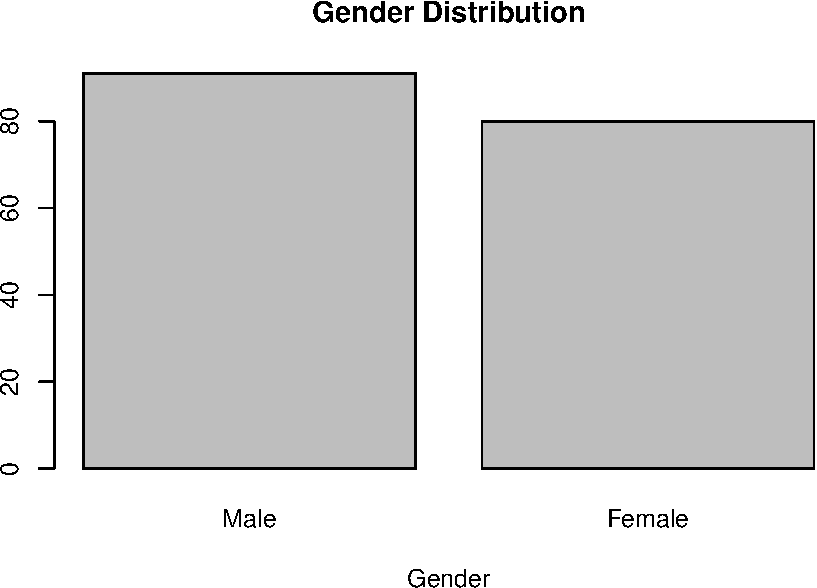
\includegraphics{Journal_files/figure-latex/unnamed-chunk-14-1.pdf}

The sample is nearly balanced by gender, yet based on this sample of the
data, there are 11 more male respondents (totaling 91) than female
respondents (totaling 80).

\emph{Use this code to draw a stacked bar plot to view the relationship
between sex and age. What can you conclude from this plot?}

\begin{Shaded}
\begin{Highlighting}[]
\NormalTok{tab.agesex }\OtherTok{\textless{}{-}} \FunctionTok{table}\NormalTok{(dat}\SpecialCharTok{$}\NormalTok{irsex, dat}\SpecialCharTok{$}\NormalTok{age2)}
\FunctionTok{barplot}\NormalTok{(tab.agesex, }\AttributeTok{main =} \StringTok{"Stacked barchart"}\NormalTok{, }\AttributeTok{xlab =} \StringTok{"Age category"}\NormalTok{, }\AttributeTok{ylab =} \StringTok{"Frequency"}\NormalTok{, }\AttributeTok{legend.text =} \FunctionTok{rownames}\NormalTok{(tab.agesex),}\AttributeTok{beside =} \ConstantTok{FALSE}\NormalTok{) }\CommentTok{\# Stacked bars (default)}
\end{Highlighting}
\end{Shaded}

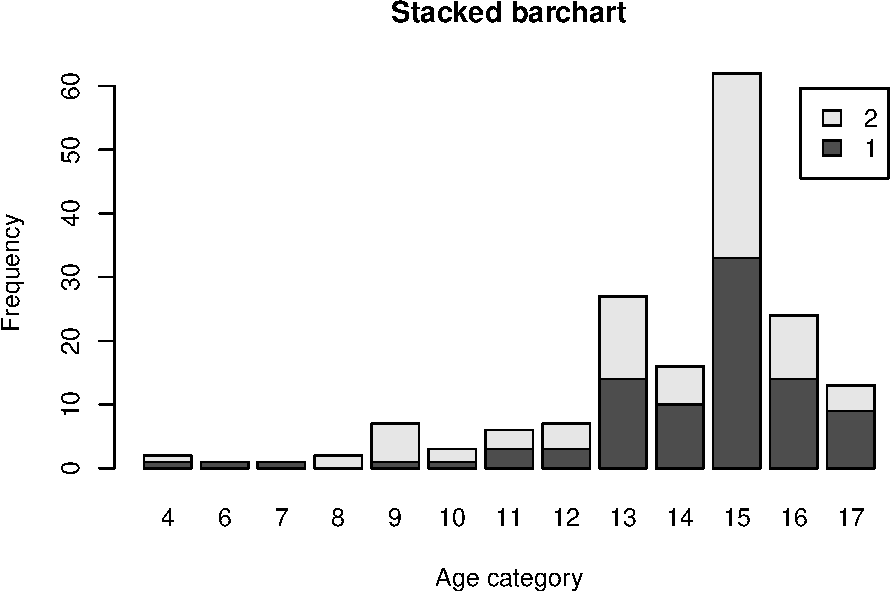
\includegraphics{Journal_files/figure-latex/unnamed-chunk-15-1.pdf}

From this plot, it is shown that the majority of individuals, both male
and female, are within the 15 age category, with gender being nearly
evenly distributed in this area. Moving to other age categories, the
outlier categories on both sides tend to be more male, while women are
more centered along the 8-16 age categories.

\hypertarget{problem-4-substance-use}{%
\subsubsection{Problem 4: Substance Use}\label{problem-4-substance-use}}

\emph{For which of the three substances included in the dataset
(marijuana, alcohol, and cigarettes) do individuals tend to use the
substance earlier?}

\begin{Shaded}
\begin{Highlighting}[]
\FunctionTok{par}\NormalTok{(}\AttributeTok{mfrow=}\FunctionTok{c}\NormalTok{(}\DecValTok{3}\NormalTok{,}\DecValTok{1}\NormalTok{))}
\FunctionTok{hist}\NormalTok{(dat}\SpecialCharTok{$}\NormalTok{mjage, }\AttributeTok{main=}\StringTok{"Histogram of Marijuana Use"}\NormalTok{, }\AttributeTok{xlab=}\StringTok{"Age of First Marijuana Use"}\NormalTok{, }\AttributeTok{ylab=}\StringTok{"Frequency"}\NormalTok{)}
\FunctionTok{hist}\NormalTok{(dat}\SpecialCharTok{$}\NormalTok{cigage, }\AttributeTok{main=}\StringTok{"Histogram of Cigarette Use"}\NormalTok{, }\AttributeTok{xlab=}\StringTok{"Age of First Cigarette Use"}\NormalTok{, }\AttributeTok{ylab=}\StringTok{"Frequency"}\NormalTok{)}
\FunctionTok{hist}\NormalTok{(dat}\SpecialCharTok{$}\NormalTok{iralcage, }\AttributeTok{main=}\StringTok{"Histogram of Alcohol Use"}\NormalTok{, }\AttributeTok{xlab=}\StringTok{"Age of First Alcohol Use"}\NormalTok{, }\AttributeTok{ylab=}\StringTok{"Frequency"}\NormalTok{)}
\end{Highlighting}
\end{Shaded}

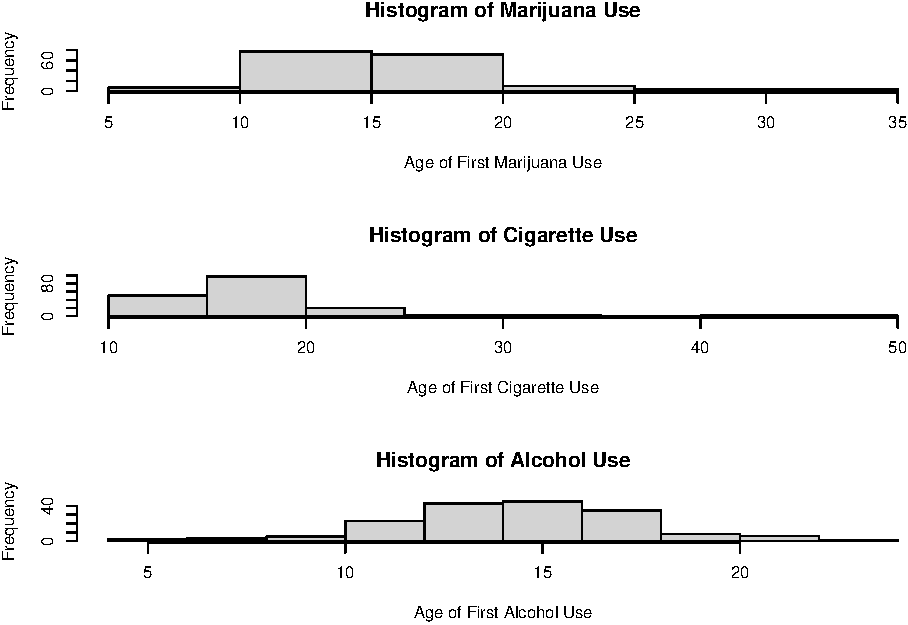
\includegraphics{Journal_files/figure-latex/unnamed-chunk-16-1.pdf}

In this dataset, marijuana is tended to be used the youngest, with a
large frequency of first use between 10-15 years of age in comparison to
the entire histogram. In the other histograms, the dispersion of first
use tends to be highest around the 15 or 15-20 age ranges.

\hypertarget{problem-5-sexual-attraction}{%
\subsubsection{Problem 5: Sexual
Attraction}\label{problem-5-sexual-attraction}}

\emph{What does the distribution of sexual attraction look like? Is this
what you expected?}

\begin{Shaded}
\begin{Highlighting}[]
\FunctionTok{as.numeric}\NormalTok{(dat}\SpecialCharTok{$}\NormalTok{sexatract)}
\end{Highlighting}
\end{Shaded}

\begin{verbatim}
##   [1]  1  2  2  1  4  4  1  1  1  1  1  1  1  1  1  1  1  1  1  1  5  1  1  5  2
##  [26]  1  1  1  1 99  1  1  1  2 99  1  1  1  1  2  1  1  1  1  2  1  1  3  1  1
##  [51]  2  1  1  1  1  1  1  1  1  1  1  3  2  1  1  3  1  1  1  1  1  1  1  1  1
##  [76]  1  1  5  1  1  1  1  1  4  1  1  2  1  1  1  1  2  2  1  1  1  6  1  1  1
## [101]  1  1  1  1  1  1  3  1  1  2  3  1  2  1  1  1  1  1  1  1  3  1  1  1  1
## [126]  1  2  3  1  1  3  1  1  1  1  1  1  1  1  1  1  1  1  1  1  1  1  1  1  1
## [151]  1  1  1  1  1  1  1  1  1  1  2  1  1  2  1  1  1  1  3  1 99
\end{verbatim}

\begin{Shaded}
\begin{Highlighting}[]
\ControlFlowTok{if}\NormalTok{ (}\SpecialCharTok{!}\FunctionTok{require}\NormalTok{(}\StringTok{\textquotesingle{}dplyr\textquotesingle{}}\NormalTok{)) }\FunctionTok{install.packages}\NormalTok{(}\StringTok{\textquotesingle{}dplyr\textquotesingle{}}\NormalTok{); }\FunctionTok{library}\NormalTok{(}\StringTok{\textquotesingle{}dplyr\textquotesingle{}}\NormalTok{)}
\NormalTok{dat}\SpecialCharTok{$}\NormalTok{sexatract }\OtherTok{\textless{}{-}}\NormalTok{ dat}\SpecialCharTok{$}\NormalTok{sexatract }\SpecialCharTok{\%\textgreater{}\%} \FunctionTok{na\_if}\NormalTok{(., }\StringTok{"99"}\NormalTok{)}
\FunctionTok{hist}\NormalTok{(dat}\SpecialCharTok{$}\NormalTok{sexatract, }\AttributeTok{main=}\StringTok{"Sexual Attraction Histogram"}\NormalTok{, }\AttributeTok{xlab =} \StringTok{"Code for Sexual Attraction"}\NormalTok{, }\AttributeTok{ylab =} \StringTok{"Frequency"}\NormalTok{)}
\end{Highlighting}
\end{Shaded}

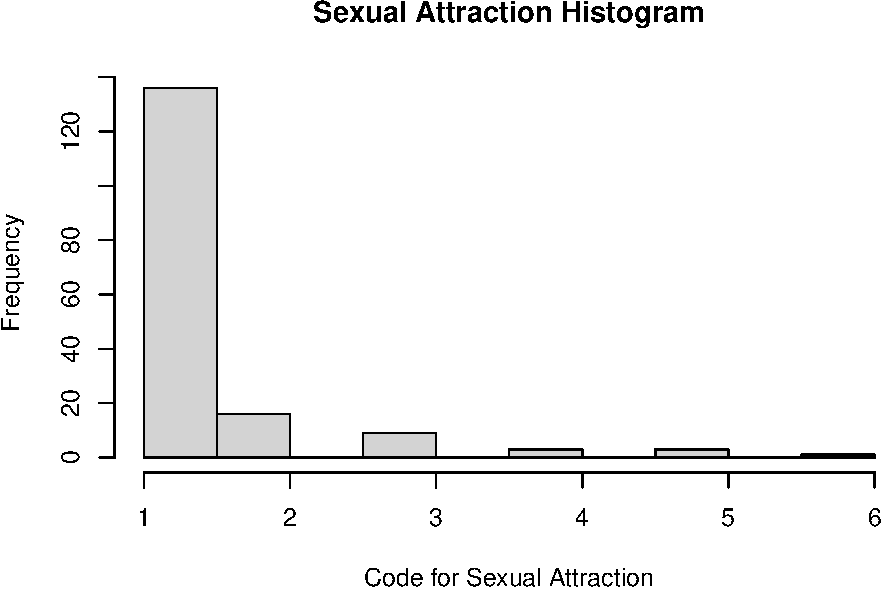
\includegraphics{Journal_files/figure-latex/unnamed-chunk-17-1.pdf}

The distribution of sexual attraction is heavily skewed to opposite-sex
attraction, under the code 1. As expected in surveying the majority of
Americans, this plot is in line with a general representation of the
population and sexuality.

\emph{What is the distribution of sexual attraction by gender?}

\begin{Shaded}
\begin{Highlighting}[]
\FunctionTok{as.numeric}\NormalTok{(dat}\SpecialCharTok{$}\NormalTok{sexatract)}
\end{Highlighting}
\end{Shaded}

\begin{verbatim}
##   [1]  1  2  2  1  4  4  1  1  1  1  1  1  1  1  1  1  1  1  1  1  5  1  1  5  2
##  [26]  1  1  1  1 NA  1  1  1  2 NA  1  1  1  1  2  1  1  1  1  2  1  1  3  1  1
##  [51]  2  1  1  1  1  1  1  1  1  1  1  3  2  1  1  3  1  1  1  1  1  1  1  1  1
##  [76]  1  1  5  1  1  1  1  1  4  1  1  2  1  1  1  1  2  2  1  1  1  6  1  1  1
## [101]  1  1  1  1  1  1  3  1  1  2  3  1  2  1  1  1  1  1  1  1  3  1  1  1  1
## [126]  1  2  3  1  1  3  1  1  1  1  1  1  1  1  1  1  1  1  1  1  1  1  1  1  1
## [151]  1  1  1  1  1  1  1  1  1  1  2  1  1  2  1  1  1  1  3  1 NA
\end{verbatim}

\begin{Shaded}
\begin{Highlighting}[]
\NormalTok{tab.atractsex }\OtherTok{\textless{}{-}} \FunctionTok{table}\NormalTok{(dat}\SpecialCharTok{$}\NormalTok{irsex, dat}\SpecialCharTok{$}\NormalTok{sexatract)}
\FunctionTok{barplot}\NormalTok{(tab.atractsex, }\AttributeTok{main =} \StringTok{"Stacked Barchart of Sexual Attraction and Sex"}\NormalTok{, }\AttributeTok{xlab =} \StringTok{"Sexual Attraction Code"}\NormalTok{, }\AttributeTok{ylab =} \StringTok{"Frequency"}\NormalTok{, }\AttributeTok{legend.text =} \FunctionTok{rownames}\NormalTok{(tab.atractsex), }\AttributeTok{beside =} \ConstantTok{FALSE}\NormalTok{) }\CommentTok{\# Stacked bars (default)}
\end{Highlighting}
\end{Shaded}

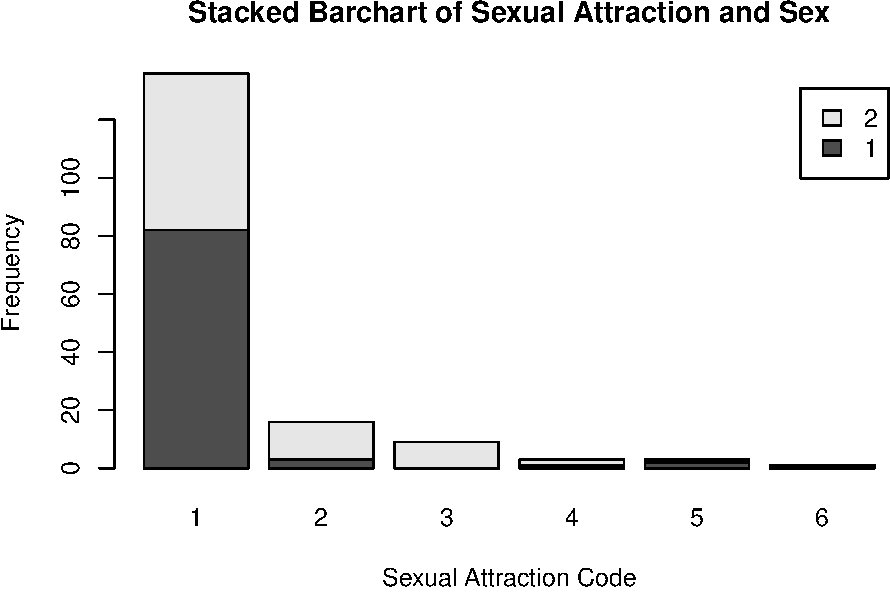
\includegraphics{Journal_files/figure-latex/unnamed-chunk-18-1.pdf}

Based on gender, men are more likely to fall under the category 1
(opposite-sex attraction), with a small proportion being strictly
homosexual. On the other hand, women tend to have more experiences in
sexual fluidity, and although the majority falls under the category 1 as
well, there is much more representation in the categories of 2, 3, and
4, signifying sexual experimentation and/or variety.

\hypertarget{problem-6-english-speaking}{%
\subsubsection{Problem 6: English
Speaking}\label{problem-6-english-speaking}}

\emph{What does the distribution of English speaking look like in the
sample? Is this what you might expect for a random sample of the US
population?}

\begin{Shaded}
\begin{Highlighting}[]
\NormalTok{tab.langsex }\OtherTok{\textless{}{-}} \FunctionTok{table}\NormalTok{(dat}\SpecialCharTok{$}\NormalTok{irsex, dat}\SpecialCharTok{$}\NormalTok{speakengl)}
\FunctionTok{barplot}\NormalTok{(tab.langsex, }\AttributeTok{main =} \StringTok{"Barchart of Sex and Language Ability"}\NormalTok{, }\AttributeTok{xlab =} \StringTok{"Language Ability"}\NormalTok{, }\AttributeTok{ylab =} \StringTok{"Frequency"}\NormalTok{, }\AttributeTok{legend.text =} \FunctionTok{rownames}\NormalTok{(tab.langsex), }\AttributeTok{beside =} \ConstantTok{FALSE}\NormalTok{) }\CommentTok{\# Stacked bars (default)}
\end{Highlighting}
\end{Shaded}

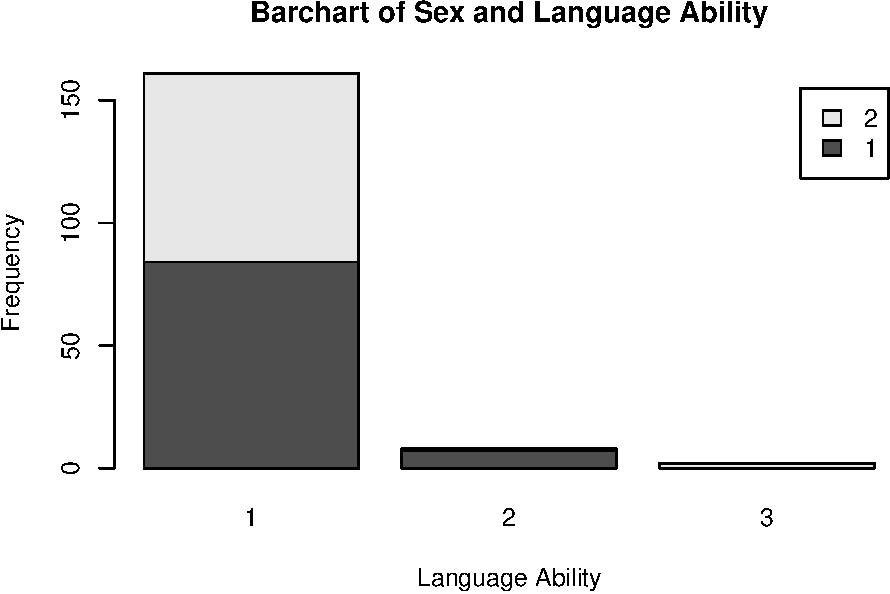
\includegraphics{Journal_files/figure-latex/unnamed-chunk-19-1.pdf}

The distribution of English ability in this sample is heavily skewed
towards 1, that of speaking English ``very well,'' nearly equally for
both males and females. However, based on the diversity of the US
population, I believe a random sample should need to include less of the
first code of perfect English and more of the codes 2, 3, and 4 in
English ability

\emph{Are there more English speaker females or males?}

\begin{Shaded}
\begin{Highlighting}[]
\NormalTok{tab.langsex}
\end{Highlighting}
\end{Shaded}

\begin{verbatim}
##    
##      1  2  3
##   1 84  7  0
##   2 77  1  2
\end{verbatim}

Here, there are a few more male English speakers than female English
speakers.

\hypertarget{exam-1}{%
\section{Exam 1}\label{exam-1}}

\hypertarget{instructions}{%
\subsubsection{Instructions}\label{instructions}}

\emph{a. Create a folder in your computer (a good place would be under
Crim 250, Exams).}

\emph{b. Download the dataset from the Canvas website
(fatal-police-shootings-data.csv) onto that folder, and save your Exam
1.Rmd file in the same folder.}

\emph{c.~Download the README.md file. This is the codebook.}

\emph{d.~Load the data into an R data frame.}

\begin{Shaded}
\begin{Highlighting}[]
\NormalTok{dat}\OtherTok{\textless{}{-}}\FunctionTok{read.csv}\NormalTok{(}\StringTok{"fatal{-}police{-}shootings{-}data.csv"}\NormalTok{)}
\FunctionTok{head}\NormalTok{(dat)}
\end{Highlighting}
\end{Shaded}

\begin{verbatim}
##   id               name       date  manner_of_death      armed age gender race
## 1  3         Tim Elliot 2015-01-02             shot        gun  53      M    A
## 2  4   Lewis Lee Lembke 2015-01-02             shot        gun  47      M    W
## 3  5 John Paul Quintero 2015-01-03 shot and Tasered    unarmed  23      M    H
## 4  8    Matthew Hoffman 2015-01-04             shot toy weapon  32      M    W
## 5  9  Michael Rodriguez 2015-01-04             shot   nail gun  39      M    H
## 6 11  Kenneth Joe Brown 2015-01-04             shot        gun  18      M    W
##            city state signs_of_mental_illness threat_level        flee
## 1       Shelton    WA                    True       attack Not fleeing
## 2         Aloha    OR                   False       attack Not fleeing
## 3       Wichita    KS                   False        other Not fleeing
## 4 San Francisco    CA                    True       attack Not fleeing
## 5         Evans    CO                   False       attack Not fleeing
## 6       Guthrie    OK                   False       attack Not fleeing
##   body_camera longitude latitude is_geocoding_exact
## 1       False  -123.122   47.247               True
## 2       False  -122.892   45.487               True
## 3       False   -97.281   37.695               True
## 4       False  -122.422   37.763               True
## 5       False  -104.692   40.384               True
## 6       False   -97.423   35.877               True
\end{verbatim}

\hypertarget{problem-1-10-points}{%
\subsubsection{Problem 1 (10 points)}\label{problem-1-10-points}}

\emph{a. Describe the dataset. This is the source:}
\emph{\url{https://github.com/washingtonpost/data-police-shootings}
.Write two sentences (max.) about this.}

The dataset describes every instance since 01/01/15 where an individual
has been fatally shot by a police officer. With this, every individual
is logged, along with the date of their death, the manner of death, if
they were armed, their age, their gender, their race, their city and
state, if there was any history of mental illness, the threat level, if
they fled, if the officer had a body camera, and the details of distance
during the shooting.

\emph{b. How many observations are there in the data frame?}

\begin{Shaded}
\begin{Highlighting}[]
\FunctionTok{head}\NormalTok{(dat)}
\end{Highlighting}
\end{Shaded}

\begin{verbatim}
##   id               name       date  manner_of_death      armed age gender race
## 1  3         Tim Elliot 2015-01-02             shot        gun  53      M    A
## 2  4   Lewis Lee Lembke 2015-01-02             shot        gun  47      M    W
## 3  5 John Paul Quintero 2015-01-03 shot and Tasered    unarmed  23      M    H
## 4  8    Matthew Hoffman 2015-01-04             shot toy weapon  32      M    W
## 5  9  Michael Rodriguez 2015-01-04             shot   nail gun  39      M    H
## 6 11  Kenneth Joe Brown 2015-01-04             shot        gun  18      M    W
##            city state signs_of_mental_illness threat_level        flee
## 1       Shelton    WA                    True       attack Not fleeing
## 2         Aloha    OR                   False       attack Not fleeing
## 3       Wichita    KS                   False        other Not fleeing
## 4 San Francisco    CA                    True       attack Not fleeing
## 5         Evans    CO                   False       attack Not fleeing
## 6       Guthrie    OK                   False       attack Not fleeing
##   body_camera longitude latitude is_geocoding_exact
## 1       False  -123.122   47.247               True
## 2       False  -122.892   45.487               True
## 3       False   -97.281   37.695               True
## 4       False  -122.422   37.763               True
## 5       False  -104.692   40.384               True
## 6       False   -97.423   35.877               True
\end{verbatim}

There are 6,594 total observations within the data frame.

\emph{c.~Look at the names of the variables in the data frame. Describe
what ``body\_camera'', ``flee'', and ``armed'' represent, according to
the codebook. Again, only write one sentence (max) per variable.}

\begin{Shaded}
\begin{Highlighting}[]
\FunctionTok{names}\NormalTok{(dat)}
\end{Highlighting}
\end{Shaded}

\begin{verbatim}
##  [1] "id"                      "name"                   
##  [3] "date"                    "manner_of_death"        
##  [5] "armed"                   "age"                    
##  [7] "gender"                  "race"                   
##  [9] "city"                    "state"                  
## [11] "signs_of_mental_illness" "threat_level"           
## [13] "flee"                    "body_camera"            
## [15] "longitude"               "latitude"               
## [17] "is_geocoding_exact"
\end{verbatim}

Within the codebook, ``body\_camera'' signifies that a news report
stated that the officer may have had a body camera on, which could have
a recording of the incident. Here, ``flee'' signifies if the individual
was moving away from the officer, either on foot, in a car, or none of
the above. Additionally, ``armed'' signifies that the victim was in
possession of an item that may have been seen as harmful by the officer.

\emph{d.~What are three weapons that you are surprised to find in the
``armed'' variable? Make a table of the values in ``armed'' to see the
options.}

\begin{Shaded}
\begin{Highlighting}[]
\FunctionTok{table}\NormalTok{(dat}\SpecialCharTok{$}\NormalTok{armed)}
\end{Highlighting}
\end{Shaded}

\begin{verbatim}
## 
##                                                   air conditioner 
##                              207                                1 
##                       air pistol                   Airsoft pistol 
##                                1                                3 
##                               ax                         barstool 
##                               24                                1 
##                     baseball bat          baseball bat and bottle 
##                               20                                1 
## baseball bat and fireplace poker           baseball bat and knife 
##                                1                                1 
##                            baton                           BB gun 
##                                6                               15 
##               BB gun and vehicle                     bean-bag gun 
##                                1                                1 
##                      beer bottle                       binoculars 
##                                3                                1 
##                     blunt object                           bottle 
##                                5                                1 
##                    bow and arrow                       box cutter 
##                                1                               13 
##                            brick              car, knife and mace 
##                                2                                1 
##                          carjack                            chain 
##                                1                                3 
##                        chain saw                         chainsaw 
##                                2                                1 
##                            chair              claimed to be armed 
##                                4                                1 
##               contractor's level                   cordless drill 
##                                1                                1 
##                         crossbow                          crowbar 
##                                9                                5 
##                        fireworks                         flagpole 
##                                1                                1 
##                       flashlight                      garden tool 
##                                2                                2 
##                      glass shard                          grenade 
##                                4                                1 
##                              gun                      gun and car 
##                             3798                               12 
##                    gun and knife                  gun and machete 
##                               22                                3 
##                    gun and sword                  gun and vehicle 
##                                1                               17 
##              guns and explosives                           hammer 
##                                3                               18 
##                       hand torch                          hatchet 
##                                1                               14 
##                  hatchet and gun                         ice pick 
##                                2                                1 
##                incendiary device                            knife 
##                                2                              955 
##                knife and vehicle                 lawn mower blade 
##                                1                                2 
##                          machete                  machete and gun 
##                               51                                1 
##                     meat cleaver                  metal hand tool 
##                                6                                2 
##                     metal object                       metal pipe 
##                                5                               16 
##                       metal pole                       metal rake 
##                                4                                1 
##                      metal stick                       microphone 
##                                3                                1 
##                       motorcycle                         nail gun 
##                                1                                1 
##                              oar                       pellet gun 
##                                1                                3 
##                              pen                     pepper spray 
##                                1                                2 
##                         pick-axe                    piece of wood 
##                                4                                7 
##                             pipe                        pitchfork 
##                                7                                2 
##                             pole                   pole and knife 
##                                3                                2 
##                  railroad spikes                             rock 
##                                1                                7 
##                    samurai sword                         scissors 
##                                4                                9 
##                      screwdriver                     sharp object 
##                               16                               14 
##                           shovel                            spear 
##                                7                                2 
##                          stapler              straight edge razor 
##                                1                                5 
##                            sword                            Taser 
##                               23                               34 
##                        tire iron                       toy weapon 
##                                4                              226 
##                          unarmed                     undetermined 
##                              421                              188 
##                   unknown weapon                          vehicle 
##                               82                              213 
##                  vehicle and gun              vehicle and machete 
##                                8                                1 
##                    walking stick                       wasp spray 
##                                1                                1 
##                           wrench 
##                                1
\end{verbatim}

Three items that I was very surprised to see that constituted as weapons
by the officer were a flashlight, a beer bottle, and wasp spray.

\hypertarget{problem-2-10-points}{%
\subsubsection{Problem 2 (10 points)}\label{problem-2-10-points}}

\emph{a. Describe the age distribution of the sample. Is this what you
would expect to see?}

\begin{Shaded}
\begin{Highlighting}[]
\FunctionTok{hist}\NormalTok{(dat}\SpecialCharTok{$}\NormalTok{age, }\AttributeTok{main=}\StringTok{"Histogram of Age"}\NormalTok{, }\AttributeTok{xlab=}\StringTok{"Age"}\NormalTok{, }\AttributeTok{ylab=}\StringTok{"Frequency"}\NormalTok{)}
\end{Highlighting}
\end{Shaded}

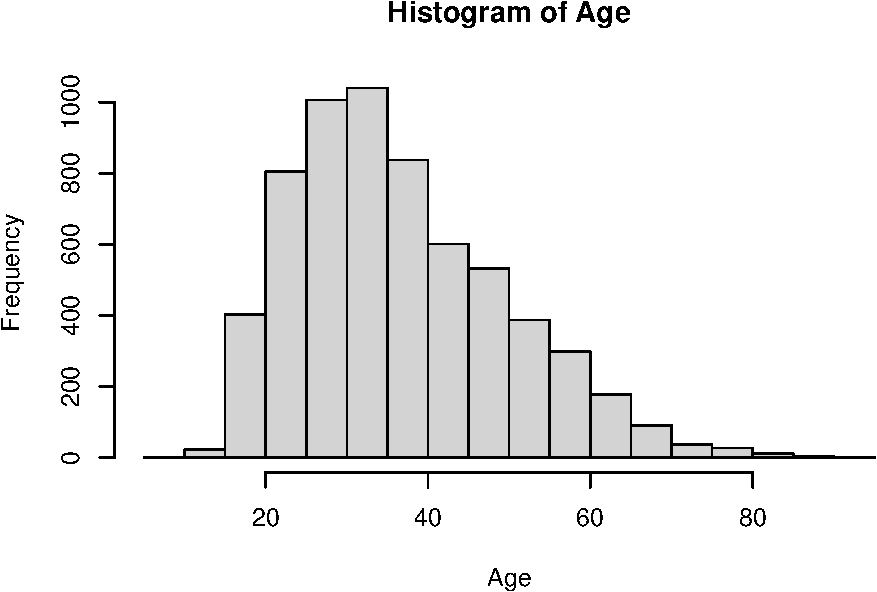
\includegraphics{Journal_files/figure-latex/unnamed-chunk-25-1.pdf}

Usually, yes, one would expect for the majority of incidents to happen
to younger individuals, somewhere in their 20's, as that reflects the
age group of individuals that may be involved in crimes the most.
However, I was surprised to see how many fatal shootings stretched into
the later years, such as those in their late 30's and into their 40's
and 60's.

\emph{b. To understand the center of the age distribution, would you use
a mean or a median, and why? Find the one you picked.}

\begin{Shaded}
\begin{Highlighting}[]
\FunctionTok{summary}\NormalTok{(dat}\SpecialCharTok{$}\NormalTok{age)}
\end{Highlighting}
\end{Shaded}

\begin{verbatim}
##    Min. 1st Qu.  Median    Mean 3rd Qu.    Max.    NA's 
##    6.00   27.00   35.00   37.12   45.00   91.00     308
\end{verbatim}

I would use the median, because the grouping of ages is unsymmetric, and
thus, the data might be skewed towards one end or the other if using the
mean. Instead of the data being skewed through the mean (plus those
unknown values skewing it more), the median would offer a better
representation of the true center of the data.

\emph{c.~Describe the gender distribution of the sample. Do you find
this surprising?}

\begin{Shaded}
\begin{Highlighting}[]
\NormalTok{dat}\SpecialCharTok{$}\NormalTok{gender.nona }\OtherTok{\textless{}{-}} \FunctionTok{na.omit}\NormalTok{(dat}\SpecialCharTok{$}\NormalTok{gender)}
\NormalTok{counts }\OtherTok{\textless{}{-}} \FunctionTok{table}\NormalTok{ (dat}\SpecialCharTok{$}\NormalTok{gender.nona)}
\FunctionTok{barplot}\NormalTok{(counts, }\AttributeTok{main=}\StringTok{"Gender Distribution"}\NormalTok{, }\AttributeTok{xlab=}\StringTok{"Gender"}\NormalTok{, }\AttributeTok{ylab=}\StringTok{"Frequency"}\NormalTok{)}
\end{Highlighting}
\end{Shaded}

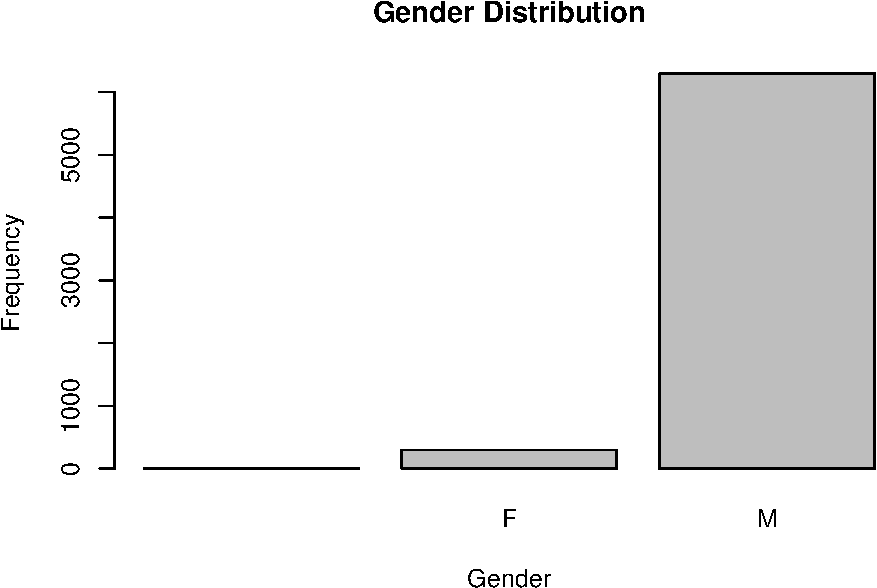
\includegraphics{Journal_files/figure-latex/unnamed-chunk-27-1.pdf}

The gender distribution of the data is heavily skewed towards male,
which is mostly aligned with what would be predicted, as the majority of
men are charged with committing crimes within the United States, and
thus, men in criminal, or fatal, situations may also be aligned with
this prediction. Although there is a small portion which seems to be of
missing values, the barplot is still undeniably skewed towards male.

\hypertarget{problem-3-10-points}{%
\subsubsection{Problem 3 (10 points)}\label{problem-3-10-points}}

\emph{a. How many police officers had a body camera, according to news
reports? What proportion is this of all the incidents in the data? Are
you surprised that it is so high or low?}

\begin{Shaded}
\begin{Highlighting}[]
\FunctionTok{table}\NormalTok{(dat}\SpecialCharTok{$}\NormalTok{body\_camera)}
\end{Highlighting}
\end{Shaded}

\begin{verbatim}
## 
## False  True 
##  5684   910
\end{verbatim}

\begin{Shaded}
\begin{Highlighting}[]
\DecValTok{910}\SpecialCharTok{/}\DecValTok{6594}
\end{Highlighting}
\end{Shaded}

\begin{verbatim}
## [1] 0.1380042
\end{verbatim}

According to news reports, 910 police officers had a body camera on
them. In relation to all of the incidents, though, it is surprising that
only 13.8\% of the officers who were involved in a fatal shooting had a
body camera on. Based on the implementation of body cameras nationwide,
one would have expected that percentage to be higher, yet it also begs
the question of the correlation between higher rates of fatal shootings
and no body cameras.

\emph{b. In how many of the incidents was the victim fleeing? What
proportion is this of the total number of incidents in the data? Is this
what you would expect?}

\begin{Shaded}
\begin{Highlighting}[]
\FunctionTok{table}\NormalTok{(dat}\SpecialCharTok{$}\NormalTok{flee)}
\end{Highlighting}
\end{Shaded}

\begin{verbatim}
## 
##                     Car        Foot Not fleeing       Other 
##         491        1058         845        3952         248
\end{verbatim}

\begin{Shaded}
\begin{Highlighting}[]
\NormalTok{(}\DecValTok{1058}\SpecialCharTok{+}\DecValTok{845}\NormalTok{)}\SpecialCharTok{/}\DecValTok{6594}
\end{Highlighting}
\end{Shaded}

\begin{verbatim}
## [1] 0.2885957
\end{verbatim}

Not including the ``other'' values, 1,903 times, or in about 28.85\% of
the instances, the victim was attempting to flee. Consequently, I would
have expected more instances of fleeing because that then implies that
while the victim was complying (at least in not fleeing) the police
officer still founds grounds to fatally shoot the individual.

\hypertarget{problem-4-10-points}{%
\subsubsection{Problem 4 (10 points)}\label{problem-4-10-points}}

\emph{a. Describe the relationship between the variables ``body camera''
and ``flee'' using a stacked barplot. What can you conclude from this
relationship?}

\emph{(Hint 1: The categories along the x-axis are the options for
``flee'', each bar contains information about whether the police officer
had a body camera (vertically), and the height along the y-axis shows
the frequency of that category.)}

\emph{(Hint 2: Also, if you are unsure about the syntax for barplot, run
?barplot in R and see some examples at the bottom of the documentation.
This is usually a good way to look up the syntax of R code. You can also
Google it.)}

\begin{Shaded}
\begin{Highlighting}[]
\NormalTok{tab.camflee }\OtherTok{\textless{}{-}} \FunctionTok{table}\NormalTok{(dat}\SpecialCharTok{$}\NormalTok{body\_camera, dat}\SpecialCharTok{$}\NormalTok{flee)}
\FunctionTok{barplot}\NormalTok{(tab.camflee, }\AttributeTok{main =} \StringTok{"Relationship of Body Camera Use and Fleeing"}\NormalTok{, }\AttributeTok{xlab =} \StringTok{"Fleeing"}\NormalTok{, }\AttributeTok{ylab =} \StringTok{"Frequency"}\NormalTok{, }\AttributeTok{legend.text =} \FunctionTok{rownames}\NormalTok{(tab.camflee), }\AttributeTok{beside =} \ConstantTok{FALSE}\NormalTok{)}
\end{Highlighting}
\end{Shaded}

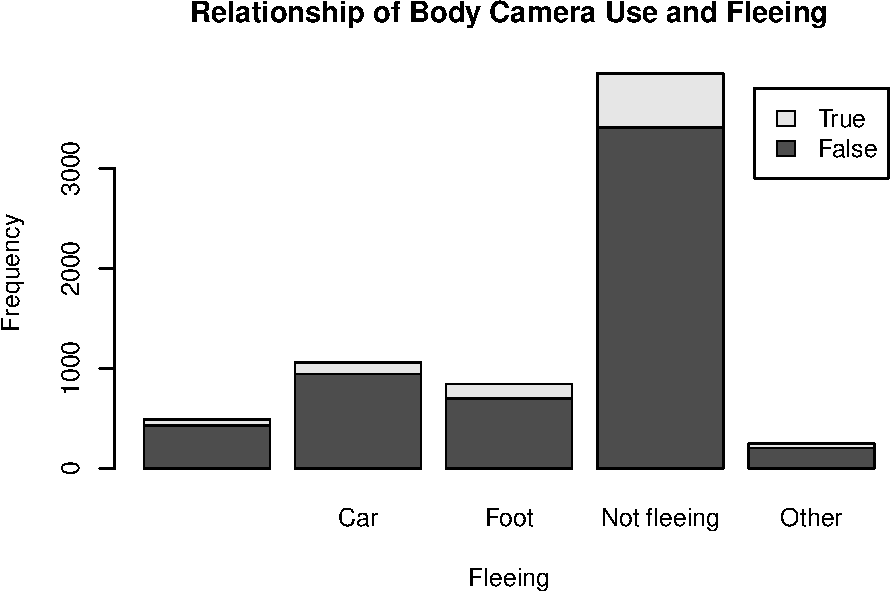
\includegraphics{Journal_files/figure-latex/unnamed-chunk-30-1.pdf}

Here, fleeing is plotted on the x axis, while the frequency of fleeing
is plotted on the y axis, while ``true'' and ``false'' on the stacked
barplots signify if a body camera was used in that exact situation. With
this relationship, one may conclude that out of all of the instances of
fleeing or not fleeing, there was more body camera usage covering that
an individual was not fleeing.

\emph{b. Describe the relationship between age and race by using a
boxplot. What can you conclude from this relationship? }

\emph{(Hint 1: The categories along the x-axis are the race categories
and the height along the y-axis is age.)}

\emph{(Hint 2: Also, if you are unsure about the syntax for boxplot, run
?boxplot in R and see some examples at the bottom of the documentation.
This is usually a good way to look up the syntax of R code. You can also
Google it.)}

\begin{Shaded}
\begin{Highlighting}[]
\FunctionTok{head}\NormalTok{(}\FunctionTok{as.numeric}\NormalTok{(dat}\SpecialCharTok{$}\NormalTok{age))}
\end{Highlighting}
\end{Shaded}

\begin{verbatim}
## [1] 53 47 23 32 39 18
\end{verbatim}

\begin{Shaded}
\begin{Highlighting}[]
\FunctionTok{suppressWarnings}\NormalTok{(}\FunctionTok{head}\NormalTok{(}\FunctionTok{as.numeric}\NormalTok{(dat}\SpecialCharTok{$}\NormalTok{race)))}
\end{Highlighting}
\end{Shaded}

\begin{verbatim}
## [1] NA NA NA NA NA NA
\end{verbatim}

\begin{Shaded}
\begin{Highlighting}[]
\NormalTok{tab.agerace }\OtherTok{\textless{}{-}} \FunctionTok{table}\NormalTok{(dat}\SpecialCharTok{$}\NormalTok{race, dat}\SpecialCharTok{$}\NormalTok{age)}
\FunctionTok{barplot}\NormalTok{(tab.agerace, }\AttributeTok{main =} \StringTok{"Relationship of Race and Age"}\NormalTok{, }\AttributeTok{xlab =} \StringTok{"Race"}\NormalTok{, }\AttributeTok{ylab =} \StringTok{"Frequency"}\NormalTok{, }\AttributeTok{legend.text =} \FunctionTok{rownames}\NormalTok{(tab.agerace), }\AttributeTok{beside =} \ConstantTok{FALSE}\NormalTok{)}
\end{Highlighting}
\end{Shaded}

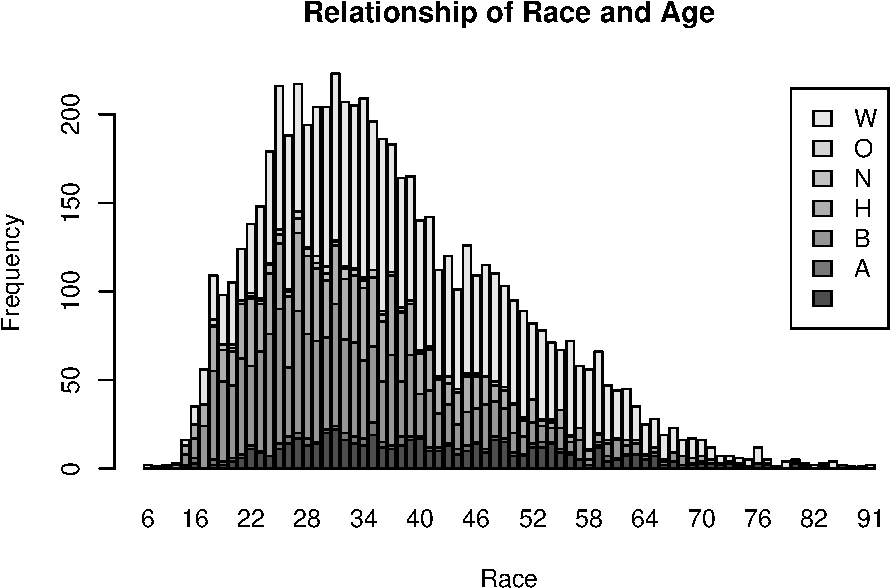
\includegraphics{Journal_files/figure-latex/unnamed-chunk-31-1.pdf}

\begin{Shaded}
\begin{Highlighting}[]
\FunctionTok{head}\NormalTok{(}\FunctionTok{as.numeric}\NormalTok{(dat}\SpecialCharTok{$}\NormalTok{age))}
\end{Highlighting}
\end{Shaded}

\begin{verbatim}
## [1] 53 47 23 32 39 18
\end{verbatim}

\begin{Shaded}
\begin{Highlighting}[]
\FunctionTok{suppressWarnings}\NormalTok{(}\FunctionTok{head}\NormalTok{(}\FunctionTok{as.numeric}\NormalTok{(dat}\SpecialCharTok{$}\NormalTok{race)))}
\end{Highlighting}
\end{Shaded}

\begin{verbatim}
## [1] NA NA NA NA NA NA
\end{verbatim}

\begin{Shaded}
\begin{Highlighting}[]
\NormalTok{tab.agerace }\OtherTok{\textless{}{-}} \FunctionTok{table}\NormalTok{(dat}\SpecialCharTok{$}\NormalTok{age, dat}\SpecialCharTok{$}\NormalTok{race)}
\FunctionTok{barplot}\NormalTok{(tab.agerace, }\AttributeTok{main =} \StringTok{"Relationship of Race and Age"}\NormalTok{, }\AttributeTok{xlab =} \StringTok{"Race"}\NormalTok{, }\AttributeTok{ylab =} \StringTok{"Frequency"}\NormalTok{, }\AttributeTok{legend.text =} \FunctionTok{rownames}\NormalTok{(tab.agerace), }\AttributeTok{beside =} \ConstantTok{FALSE}\NormalTok{)}
\end{Highlighting}
\end{Shaded}

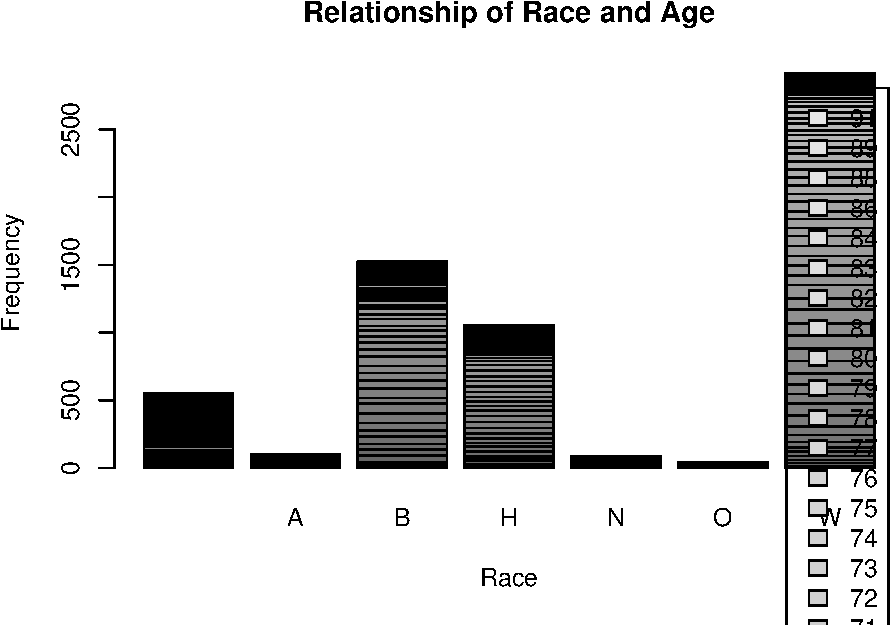
\includegraphics{Journal_files/figure-latex/unnamed-chunk-31-2.pdf}

Plotting age and race both ways, the first graph demonstrates ages along
the x axis and frequency along the y axis, with the key representing
different races. The second graph demonstrates race along the x axis,
frequency along the y axis, and ages within the key. Here, it is shown
that the majority of fatal shooting victims are indeed white, with
African Americans coming as the second highest grouping for victims,
with the majority of both being within the age ranges of 26-36 years
old.

\hypertarget{extra-credit-10-points}{%
\subsubsection{Extra credit (10 points)}\label{extra-credit-10-points}}

\emph{a. What does this code tell us?}

\begin{Shaded}
\begin{Highlighting}[]
\NormalTok{mydates }\OtherTok{\textless{}{-}} \FunctionTok{as.Date}\NormalTok{(dat}\SpecialCharTok{$}\NormalTok{date)}
\FunctionTok{head}\NormalTok{(mydates)}
\NormalTok{(mydates[}\FunctionTok{length}\NormalTok{(mydates)] }\SpecialCharTok{{-}}\NormalTok{ mydates[}\DecValTok{1}\NormalTok{])}
\end{Highlighting}
\end{Shaded}

The code explains how much of a time difference there was between all
occurances of fatal shootings, with the difference being 2,458 days
total.

\emph{b. On Friday, a new report was published that was described as
follows by The Guardian: ``More than half of US police killings are
mislabelled or not reported, study finds.'' Without reading this article
now (due to limited time), why do you think police killings might be
mislabelled or underreported?}

Police killings might be mislabeled or underreported first due to
processing issues, where an officer might not process the report
properly, the report may not have all necessary information, or
different processors may not have investigated the event thoroughly.
Second, officers who may be liable for a wrongly death may not report
the incident, or even do so correctly. Third, with a wrongly death, an
officer may report that the victim had a weapon in his hand, or that he
was fleeing, when he truly was not, in order to grant the officer
clemency for the situation.

\emph{c.~Regarding missing values in problem 4, do you see any? If so,
do you think that's all that's missing from the data?}

In section a of problem 4, there are many missing values within the
``fleeing'' variable, off to the left side of the graph, where there is
no data if the victim fled or not. There is simply a bar determining if
there was a body camera during the situation or not. Additionally, the
``other'' portion is unspecified as to what ``other'' may be, thus
causing more vagueness in the results of the data. With this data, I
believe not only are there missing values to it, but the vagueness of
the ``other'' section leads to more missing values and less
understanding of the situation based on if the victim was fleeing or not
(and how).

\hypertarget{assignment-3}{%
\section{Assignment 3}\label{assignment-3}}

\begin{Shaded}
\begin{Highlighting}[]
\NormalTok{knitr}\SpecialCharTok{::}\NormalTok{opts\_chunk}\SpecialCharTok{$}\FunctionTok{set}\NormalTok{(}\AttributeTok{echo =} \ConstantTok{TRUE}\NormalTok{)}
\end{Highlighting}
\end{Shaded}

Submit your responses as either an HTML file or a PDF file on Canvas.
Also, please upload it to your website.

Load the data.

\begin{Shaded}
\begin{Highlighting}[]
\FunctionTok{library}\NormalTok{(readr)}
\FunctionTok{library}\NormalTok{(knitr)}
\NormalTok{dat.crime }\OtherTok{\textless{}{-}} \FunctionTok{read\_delim}\NormalTok{(}\StringTok{"crime\_simple.txt"}\NormalTok{, }\AttributeTok{delim =} \StringTok{"}\SpecialCharTok{\textbackslash{}t}\StringTok{"}\NormalTok{)}
\end{Highlighting}
\end{Shaded}

This is a dataset from a textbook by Brian S. Everitt about crime in the
US in 1960. The data originate from the Uniform Crime Report of the FBI
and other government sources. The data for 47 states of the USA are
given.

\hypertarget{codebook}{%
\subparagraph{Codebook:}\label{codebook}}

\emph{R}: Crime rate: \# of offenses reported to police per million
population

\emph{Age}: The number of males of age 14-24 per 1000 population

\emph{S}: Indicator variable for Southern states (0 = No, 1 = Yes)

\emph{Ed}: Mean of years of schooling x 10 for persons of age 25 or
older

\emph{Ex0}: 1960 per capita expenditure on police by state and local
government

\emph{Ex1}: 1959 per capita expenditure on police by state and local
government

\emph{LF}: Labor force participation rate per 1000 civilian urban males
age 14-24

\emph{M}: The number of males per 1000 females

\emph{N}: State population size in hundred thousands

\emph{NW}: The number of non-whites per 1000 population

\emph{U1}: Unemployment rate of urban males per 1000 of age 14-24

\emph{U2}: Unemployment rate of urban males per 1000 of age 35-39

\emph{W}: Median value of transferable goods and assets or family income
in tens of \$

\emph{X}: The number of families per 1000 earning below 1/2 the median
income

We are interested in checking whether the reported crime rate (\# of
offenses reported to police per million population) and the average
education (mean number of years of schooling for persons of age 25 or
older) are related.

\textbf{1. How many observations are there in the dataset? To what does
each observation correspond?}

\begin{Shaded}
\begin{Highlighting}[]
\NormalTok{dat.crime}
\end{Highlighting}
\end{Shaded}

\begin{verbatim}
## # A tibble: 47 x 14
##        R   Age     S    Ed   Ex0   Ex1    LF     M     N    NW    U1    U2     W
##    <dbl> <dbl> <dbl> <dbl> <dbl> <dbl> <dbl> <dbl> <dbl> <dbl> <dbl> <dbl> <dbl>
##  1  79.1   151     1    91    58    56   510   950    33   301   108    41   394
##  2 164.    143     0   113   103    95   583  1012    13   102    96    36   557
##  3  57.8   142     1    89    45    44   533   969    18   219    94    33   318
##  4 197.    136     0   121   149   141   577   994   157    80   102    39   673
##  5 123.    141     0   121   109   101   591   985    18    30    91    20   578
##  6  68.2   121     0   110   118   115   547   964    25    44    84    29   689
##  7  96.3   127     1   111    82    79   519   982     4   139    97    38   620
##  8 156.    131     1   109   115   109   542   969    50   179    79    35   472
##  9  85.6   157     1    90    65    62   553   955    39   286    81    28   421
## 10  70.5   140     0   118    71    68   632  1029     7    15   100    24   526
## # ... with 37 more rows, and 1 more variable: X <dbl>
\end{verbatim}

There are 47 total observations within the dataset, with each
observation representing a state within the United States of America,
excluding three remaining states.

\textbf{2. Draw a scatterplot of the two variables. Calculate the
correlation between the two variables. Can you come up with an
explanation for this relationship?}

\begin{Shaded}
\begin{Highlighting}[]
\FunctionTok{library}\NormalTok{(datasets)}
\FunctionTok{plot}\NormalTok{(dat.crime}\SpecialCharTok{$}\NormalTok{R, dat.crime}\SpecialCharTok{$}\NormalTok{Ed,  }\AttributeTok{main=}\StringTok{"Relationship between Reported Crime Rate and Average Education"}\NormalTok{,}
    \AttributeTok{xlab=}\StringTok{"Criminal Offenses per Million"}\NormalTok{, }\AttributeTok{ylab=}\StringTok{"Mean Schooling Years for Individuals Aged 25+"}\NormalTok{)}


\FunctionTok{library}\NormalTok{(datasets)}
\NormalTok{reg.output.nc }\OtherTok{\textless{}{-}} \FunctionTok{lm}\NormalTok{(}\AttributeTok{formula =}\NormalTok{ Ed }\SpecialCharTok{\textasciitilde{}}\NormalTok{ R, }\AttributeTok{data =}\NormalTok{ dat.crime)}
\FunctionTok{plot}\NormalTok{(dat.crime}\SpecialCharTok{$}\NormalTok{R, dat.crime}\SpecialCharTok{$}\NormalTok{Ed,  }\AttributeTok{main=}\StringTok{"Relationship between Reported Crime Rate and Average Education"}\NormalTok{,}
    \AttributeTok{xlab=}\StringTok{"Criminal Offenses per Million"}\NormalTok{, }\AttributeTok{ylab=}\StringTok{"Mean Schooling Years for Individuals Aged 25+"}\NormalTok{)}
\FunctionTok{abline}\NormalTok{(reg.output.nc, }\AttributeTok{col=}\StringTok{"blue"}\NormalTok{)}
\end{Highlighting}
\end{Shaded}

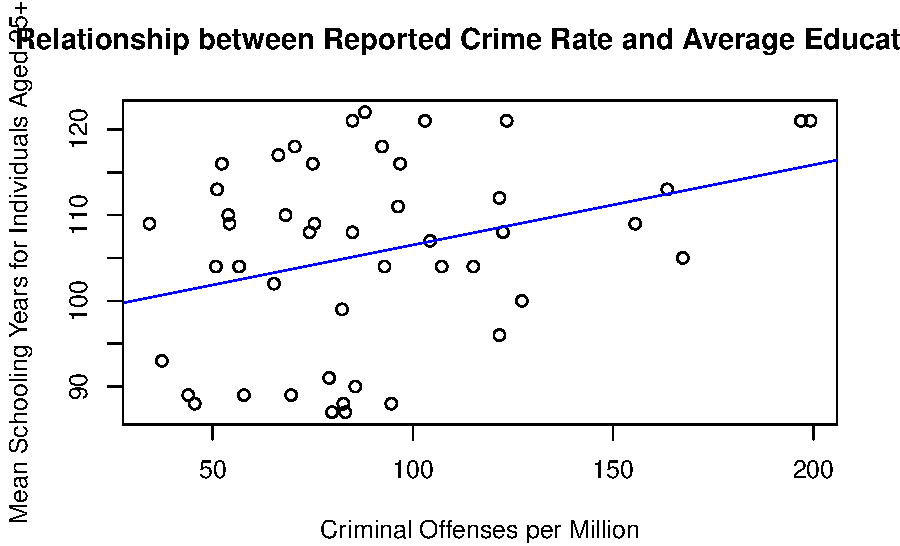
\includegraphics{Journal_files/figure-latex/unnamed-chunk-36-1.pdf}

\begin{Shaded}
\begin{Highlighting}[]
\FunctionTok{cor}\NormalTok{(dat.crime}\SpecialCharTok{$}\NormalTok{R, dat.crime}\SpecialCharTok{$}\NormalTok{Ed)}
\end{Highlighting}
\end{Shaded}

\begin{verbatim}
## [1] 0.3228349
\end{verbatim}

The correlation within this scatterplot is faintly a positive
correlation of 0.3228349. This relationship, thus, may be explained as
having an extremely weak positive correlation, leaning more towards no
correlation, between education rates and criminal offenses. Thus,
reports of criminal offenses may occur with both a lower and somewhat
higher education rate.

\textbf{3. Regress reported crime rate (y) on average education (x) and
call this linear model \texttt{crime.lm} and write the summary of the
regression.}

\begin{Shaded}
\begin{Highlighting}[]
\NormalTok{dat.crime}\SpecialCharTok{$}\NormalTok{R.c }\OtherTok{=} \FunctionTok{scale}\NormalTok{(dat.crime}\SpecialCharTok{$}\NormalTok{R, }\AttributeTok{center=}\ConstantTok{TRUE}\NormalTok{, }\AttributeTok{scale=}\ConstantTok{FALSE}\NormalTok{)}
\NormalTok{crime.lm }\OtherTok{\textless{}{-}} \FunctionTok{lm}\NormalTok{(}\AttributeTok{formula =}\NormalTok{ Ed }\SpecialCharTok{\textasciitilde{}}\NormalTok{ dat.crime}\SpecialCharTok{$}\NormalTok{R.c, }\AttributeTok{data =}\NormalTok{ dat.crime) }
\FunctionTok{summary}\NormalTok{(crime.lm) }
\end{Highlighting}
\end{Shaded}

\begin{verbatim}
## 
## Call:
## lm(formula = Ed ~ dat.crime$R.c, data = dat.crime)
## 
## Residuals:
##     Min      1Q  Median      3Q     Max 
## -18.020  -8.441   1.528   8.200  16.596 
## 
## Coefficients:
##                Estimate Std. Error t value Pr(>|t|)    
## (Intercept)   105.63830    1.56148  67.653   <2e-16 ***
## dat.crime$R.c   0.09338    0.04081   2.288   0.0269 *  
## ---
## Signif. codes:  0 '***' 0.001 '**' 0.01 '*' 0.05 '.' 0.1 ' ' 1
## 
## Residual standard error: 10.7 on 45 degrees of freedom
## Multiple R-squared:  0.1042, Adjusted R-squared:  0.08432 
## F-statistic: 5.236 on 1 and 45 DF,  p-value: 0.02688
\end{verbatim}

\textbf{4. Are the four assumptions of linear regression satisfied? To
answer this, draw the relevant plots. (Write a maximum of one sentence
per assumption.)}

\begin{Shaded}
\begin{Highlighting}[]
\FunctionTok{plot}\NormalTok{(dat.crime}\SpecialCharTok{$}\NormalTok{R.c, crime.lm}\SpecialCharTok{$}\NormalTok{residuals, }\AttributeTok{ylim=}\FunctionTok{c}\NormalTok{(}\SpecialCharTok{{-}}\DecValTok{15}\NormalTok{,}\DecValTok{15}\NormalTok{), }\AttributeTok{main=}\StringTok{"Residuals vs. x"}\NormalTok{, }\AttributeTok{xlab=}\StringTok{"x, Scaled Reported Crime"}\NormalTok{, }\AttributeTok{ylab=}\StringTok{"Residuals"}\NormalTok{)}
\FunctionTok{abline}\NormalTok{(}\AttributeTok{h =} \DecValTok{0}\NormalTok{, }\AttributeTok{lty=}\StringTok{"dashed"}\NormalTok{)}
\end{Highlighting}
\end{Shaded}

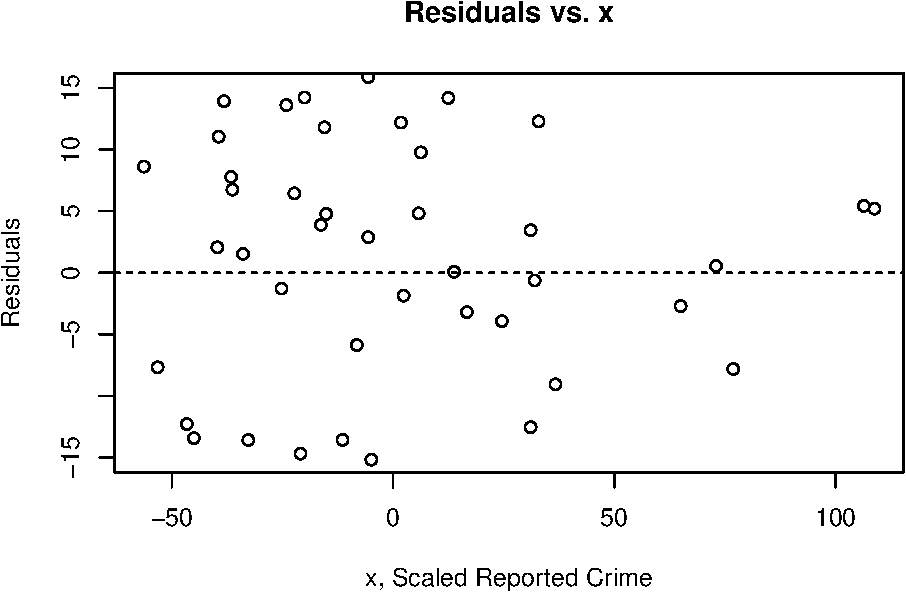
\includegraphics{Journal_files/figure-latex/unnamed-chunk-38-1.pdf}

\begin{Shaded}
\begin{Highlighting}[]
\FunctionTok{plot}\NormalTok{(crime.lm, }\AttributeTok{which=}\DecValTok{1}\NormalTok{)}
\end{Highlighting}
\end{Shaded}

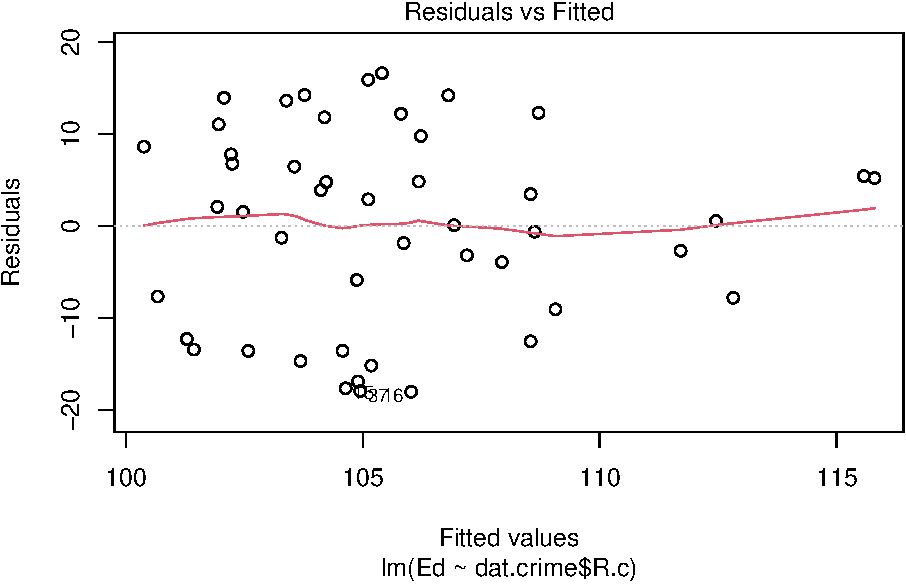
\includegraphics{Journal_files/figure-latex/unnamed-chunk-38-2.pdf}

\begin{Shaded}
\begin{Highlighting}[]
\FunctionTok{plot}\NormalTok{(crime.lm, }\AttributeTok{which=}\DecValTok{3}\NormalTok{)}
\end{Highlighting}
\end{Shaded}

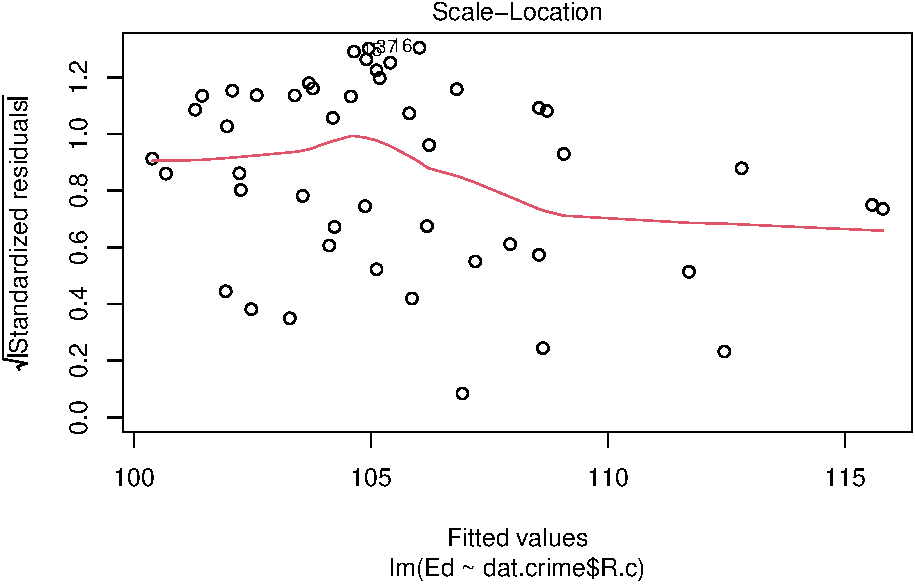
\includegraphics{Journal_files/figure-latex/unnamed-chunk-38-3.pdf}

\begin{Shaded}
\begin{Highlighting}[]
\FunctionTok{plot}\NormalTok{(crime.lm, }\AttributeTok{which=}\DecValTok{5}\NormalTok{)}
\end{Highlighting}
\end{Shaded}

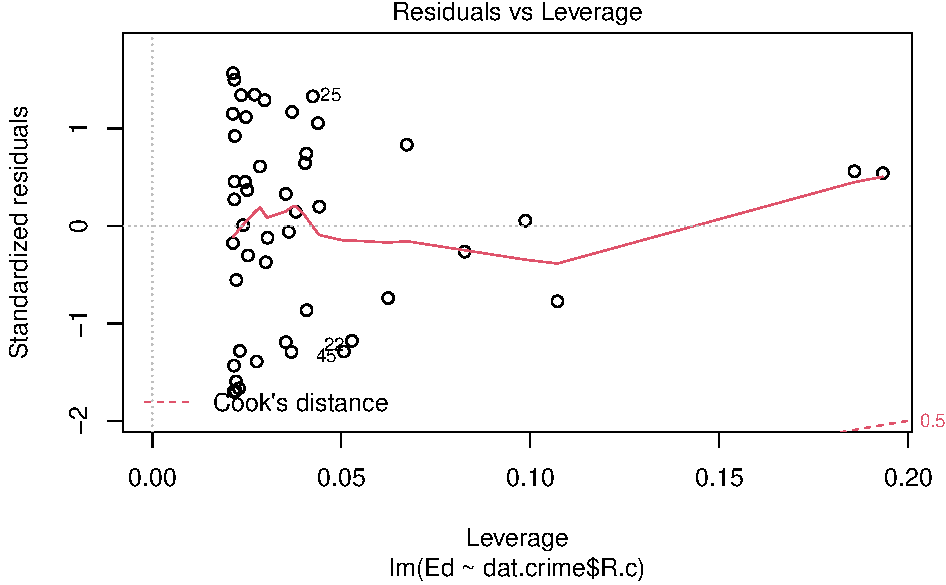
\includegraphics{Journal_files/figure-latex/unnamed-chunk-38-4.pdf}

\begin{Shaded}
\begin{Highlighting}[]
\FunctionTok{plot}\NormalTok{(crime.lm, }\AttributeTok{which=}\DecValTok{2}\NormalTok{)}
\end{Highlighting}
\end{Shaded}

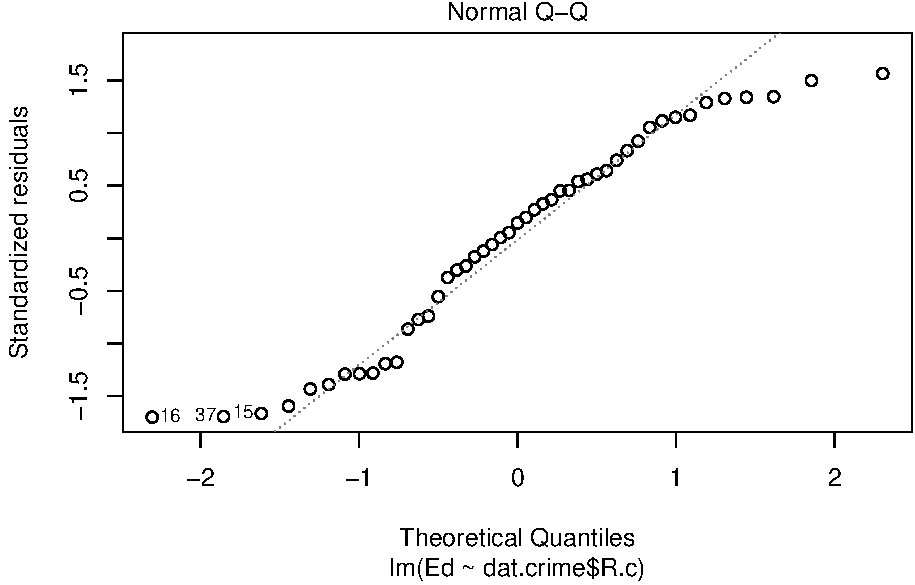
\includegraphics{Journal_files/figure-latex/unnamed-chunk-38-5.pdf}

Dealing with the four assumptions of linear regression, the first two
assumptions of linearity and independence may be demonstrated through
the first plots of residuals vs.~x and residuals vs.~fitted, where both
assumptions hold true. Within the first two plots, linearity is true
through the horizontal direction of the plot, and independence is true
through no evidence of patterns that may constitute clumpings which
diminish independence. Next, the third assumption of homoscedasticity is
proved true through the scale-location plot, where there is no
significant trend leading to a non-constant variance. Last, the fourth
assumption of normal population is proved true in both a residuals
vs.~leverage plot and normal qq plot, where there are no significant
outliers or significantly heavy skews, respectively.

\textbf{5. Is the relationship between reported crime and average
education statistically significant? Report the estimated coefficient of
the slope, the standard error, and the p-value. What does it mean for
the relationship to be statistically significant?}

\begin{Shaded}
\begin{Highlighting}[]
\FunctionTok{summary}\NormalTok{(crime.lm) }
\end{Highlighting}
\end{Shaded}

\begin{verbatim}
## 
## Call:
## lm(formula = Ed ~ dat.crime$R.c, data = dat.crime)
## 
## Residuals:
##     Min      1Q  Median      3Q     Max 
## -18.020  -8.441   1.528   8.200  16.596 
## 
## Coefficients:
##                Estimate Std. Error t value Pr(>|t|)    
## (Intercept)   105.63830    1.56148  67.653   <2e-16 ***
## dat.crime$R.c   0.09338    0.04081   2.288   0.0269 *  
## ---
## Signif. codes:  0 '***' 0.001 '**' 0.01 '*' 0.05 '.' 0.1 ' ' 1
## 
## Residual standard error: 10.7 on 45 degrees of freedom
## Multiple R-squared:  0.1042, Adjusted R-squared:  0.08432 
## F-statistic: 5.236 on 1 and 45 DF,  p-value: 0.02688
\end{verbatim}

Based on the single asterisk next to the slope's p-value, but three
significant asterisks near the intercept's p-value, it is difficult to
discern whether the relationship is statistically significant. Taking
the significance of the intercept's p-value against that of the slope,
they may be averaged to display a slight significance of the data
between reported crime and education level, with significance meaning
that the result is unlikely to occur under a null hypothesis. However,
there is no discernible rejection of the null hypothesis within the data
results. Dealing with solely the slope, the estimated coefficient is
0.09338, the standard error is 0.04081, and the p-value is 0.0269.

\textbf{6. How are reported crime and average education related? In
other words, for every unit increase in average education, how does
reported crime rate change (per million) per state?}

\begin{Shaded}
\begin{Highlighting}[]
\NormalTok{crime.lm}\SpecialCharTok{$}\NormalTok{coefficients}
\end{Highlighting}
\end{Shaded}

\begin{verbatim}
##   (Intercept) dat.crime$R.c 
##  105.63829787    0.09337905
\end{verbatim}

Here, with slope described as a unit increase in one variable per unit
increase in a second variable, the slope would signify that there is an
increase in crime reports by 0.09337905 per million with each unit of
increase in average education.

\textbf{7. Can you conclude that if individuals were to receive more
education, then crime will be reported more often? Why or why not?}

It is difficult to discern or state that there is a positive correlation
between education and crime reports, for it is an extremely weak
correlation between the two, with a correlation estimate rounding to
only about 0.3. Although the plots comparing crime reports and education
were proven to be accurate plots through the four assumptions, the
extremely low-valued slope, the insignificant p-value of the slope, and
no true proof of rejection of the null hypothesis lead an observer to
believe that there is no true correlation between the two. Thus, if
individuals were to receive more education, it is not discernible to say
that crime will also be reported more often.

\hypertarget{exam-2}{%
\section{Exam 2}\label{exam-2}}

\begin{enumerate}
\def\labelenumi{\alph{enumi}.}
\item
  Create a folder in your computer (a good place would be under Crim
  250, Exams).
\item
  Download the dataset from the Canvas website (sim.data.csv) onto that
  folder, and save your Exam 2.Rmd file in the same folder.
\item
  Data description: This dataset provides (simulated) data about 200
  police departments in one year. It contains information about the
  funding received by the department as well as incidents of police
  brutality. Suppose this dataset (sim.data.csv) was collected by
  researchers to answer this question: \textbf{``Does having more
  funding in a police department lead to fewer incidents of police
  brutality?''}
\item
  Codebook:
\end{enumerate}

\begin{itemize}
\tightlist
\item
  funds: How much funding the police department received in that year in
  millions of dollars.
\item
  po.brut: How many incidents of police brutality were reported by the
  department that year.
\item
  po.dept.code: Police department code
\end{itemize}

\hypertarget{problem-1-eda-10-points}{%
\subsection{Problem 1: EDA (10 points)}\label{problem-1-eda-10-points}}

\emph{Describe the dataset and variables. Perform exploratory data
analysis for the two variables of interest: funds and po.brut.}

\begin{Shaded}
\begin{Highlighting}[]
\NormalTok{dat}\OtherTok{\textless{}{-}}\FunctionTok{read.csv}\NormalTok{(}\AttributeTok{file =} \StringTok{\textquotesingle{}sim.data.csv\textquotesingle{}}\NormalTok{)}
\FunctionTok{head}\NormalTok{(dat)}
\end{Highlighting}
\end{Shaded}

\begin{verbatim}
##   po.dept.code funds po.brut
## 1            1  48.1      23
## 2            2  81.4      10
## 3            3  41.8      25
## 4            4  61.7      19
## 5            5  86.4       8
## 6            6  51.6      22
\end{verbatim}

\begin{Shaded}
\begin{Highlighting}[]
\FunctionTok{names}\NormalTok{(dat)}
\end{Highlighting}
\end{Shaded}

\begin{verbatim}
## [1] "po.dept.code" "funds"        "po.brut"
\end{verbatim}

\begin{Shaded}
\begin{Highlighting}[]
\FunctionTok{plot}\NormalTok{(dat}\SpecialCharTok{$}\NormalTok{funds, dat}\SpecialCharTok{$}\NormalTok{po.brut, }\AttributeTok{main =} \StringTok{"Relationship Between Police Funding (in millions) and Brutality Incidents"}\NormalTok{, }\AttributeTok{xlab =} \StringTok{"Police Funding (in millions"}\NormalTok{, }\AttributeTok{ylab =} \StringTok{"Police Brutality Incidents"}\NormalTok{)}
\end{Highlighting}
\end{Shaded}

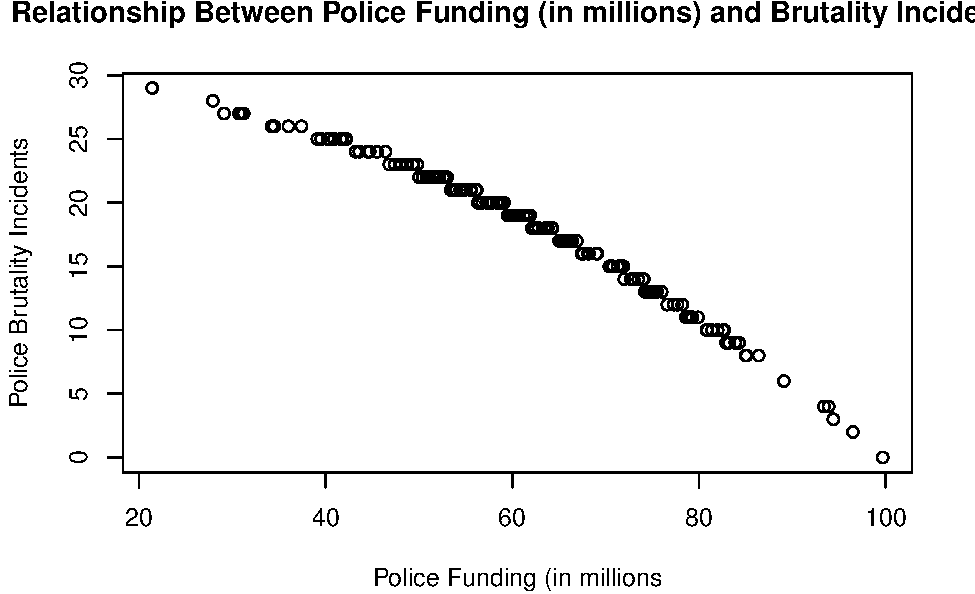
\includegraphics{Journal_files/figure-latex/unnamed-chunk-41-1.pdf}

Here, the dataset describes a simulated account of 200 police
departments, where in each department, their allocated funding (in
millions) and the number of police brutality incidents within that
police department are compared within a singular year. Within the
dataset, the variables include the police department's code, the yearly
funds allocated to them in millions, and the number of police brutality
incidents they had within a year.

Here, the EDA of the data, within a scatterplot, demostrates a strong
correlation between higher funding and lower brutality incidents.

\hypertarget{problem-2-linear-regression-30-points}{%
\subsection{Problem 2: Linear regression (30
points)}\label{problem-2-linear-regression-30-points}}

\emph{a. Perform a simple linear regression to answer the question of
interest. To do this, name your linear model ``reg.output'' and write
the summary of the regression by using ``summary(reg.output)''.}

\begin{Shaded}
\begin{Highlighting}[]
\NormalTok{reg.output }\OtherTok{\textless{}{-}} \FunctionTok{lm}\NormalTok{(}\AttributeTok{formula =}\NormalTok{ dat}\SpecialCharTok{$}\NormalTok{po.brut }\SpecialCharTok{\textasciitilde{}}\NormalTok{ dat}\SpecialCharTok{$}\NormalTok{funds, }\AttributeTok{data =}\NormalTok{ dat)}
\FunctionTok{plot}\NormalTok{(dat}\SpecialCharTok{$}\NormalTok{funds, dat}\SpecialCharTok{$}\NormalTok{po.brut, }\AttributeTok{main =} \StringTok{"Linear Regression of Police Funding and Police Brutality"}\NormalTok{, }\AttributeTok{xlab =} \StringTok{"Department Funding in Millions"}\NormalTok{, }\AttributeTok{ylab =} \StringTok{"Police Brutality Incidents"}\NormalTok{)}
\FunctionTok{abline}\NormalTok{(reg.output, }\AttributeTok{col=}\StringTok{"blue"}\NormalTok{)}
\end{Highlighting}
\end{Shaded}

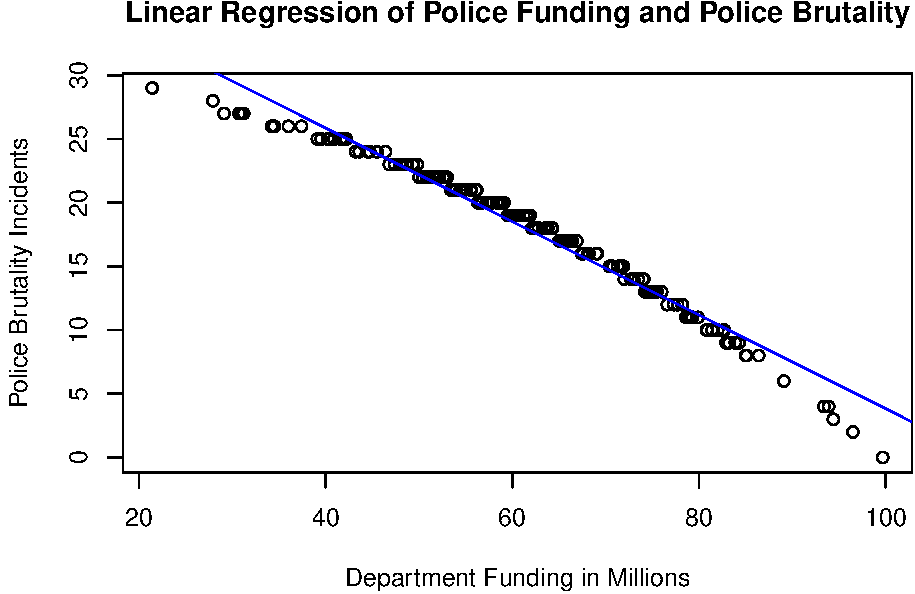
\includegraphics{Journal_files/figure-latex/unnamed-chunk-42-1.pdf}

\begin{Shaded}
\begin{Highlighting}[]
\FunctionTok{summary}\NormalTok{(reg.output)}
\end{Highlighting}
\end{Shaded}

\begin{verbatim}
## 
## Call:
## lm(formula = dat$po.brut ~ dat$funds, data = dat)
## 
## Residuals:
##     Min      1Q  Median      3Q     Max 
## -3.9433 -0.2233  0.2544  0.5952  1.1803 
## 
## Coefficients:
##              Estimate Std. Error t value Pr(>|t|)    
## (Intercept) 40.543069   0.282503  143.51   <2e-16 ***
## dat$funds   -0.367099   0.004496  -81.64   <2e-16 ***
## ---
## Signif. codes:  0 '***' 0.001 '**' 0.01 '*' 0.05 '.' 0.1 ' ' 1
## 
## Residual standard error: 0.9464 on 198 degrees of freedom
## Multiple R-squared:  0.9712, Adjusted R-squared:  0.971 
## F-statistic:  6666 on 1 and 198 DF,  p-value: < 2.2e-16
\end{verbatim}

\begin{Shaded}
\begin{Highlighting}[]
\FunctionTok{cor}\NormalTok{(dat}\SpecialCharTok{$}\NormalTok{funds, dat}\SpecialCharTok{$}\NormalTok{po.brut)}
\end{Highlighting}
\end{Shaded}

\begin{verbatim}
## [1] -0.9854706
\end{verbatim}

Regarding the main question, there seems to be a strong correlation
between having more department funding and experiencing less incidents
of police brutality, where less deparment funding generally leads to
much higher rates of police brutality incidents. Here, the line of best
fit also demonstrates this extremely strong negative correlation.

\emph{b. Report the estimated coefficient, standard error, and p-value
of the slope. Is the relationship between funds and incidents
statistically significant? Explain.}

Here, the estimated coefficient of the slope is -0.367099, the standard
error of the slope is 0.004496, and the p-value of the slope is
\textless2e-16. Observing these values, the relationship between funds
and incidents is statistically significant, as the p-value of the slope
is much smaller than the alpha at 0.05 (which leads to the rejection of
the null hypothesis), the p-value of the slope has three asterisks of
significance, and the correlation reaches a value of -98.5\%.

\emph{c.~Draw a scatterplot of po.brut (y-axis) and funds (x-axis).
Right below your plot command, use abline to draw the fitted regression
line, like this:}

\begin{Shaded}
\begin{Highlighting}[]
\FunctionTok{plot}\NormalTok{(dat}\SpecialCharTok{$}\NormalTok{funds, dat}\SpecialCharTok{$}\NormalTok{po.brut, }\AttributeTok{main =} \StringTok{"Linear Regression of Police Funding and Police Brutality"}\NormalTok{, }\AttributeTok{xlab =} \StringTok{"Department Funding in Millions"}\NormalTok{, }\AttributeTok{ylab =} \StringTok{"Police Brutality Incidents"}\NormalTok{)}
\FunctionTok{abline}\NormalTok{(reg.output, }\AttributeTok{col =} \StringTok{"red"}\NormalTok{, }\AttributeTok{lwd=}\DecValTok{2}\NormalTok{)}
\end{Highlighting}
\end{Shaded}

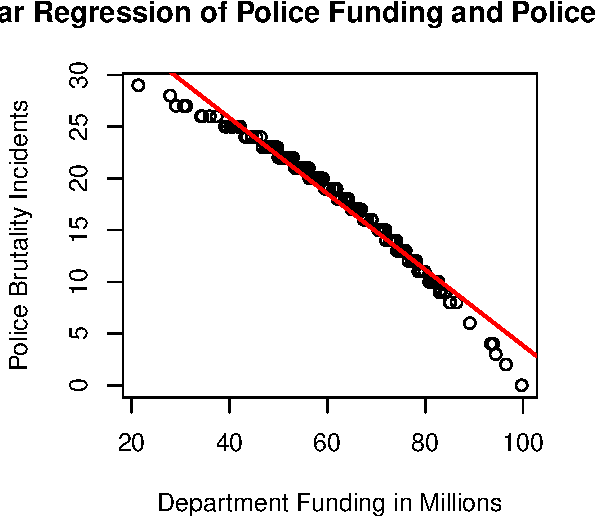
\includegraphics{Journal_files/figure-latex/unnamed-chunk-43-1.pdf}

\emph{Does the line look like a good fit? Why or why not?}

Yes, the line does look like a good fit, as there is only a slight skew
between the actual scatterplot and the line of best fit. Comparing the
values, there is a high correlation between the values in the middle and
the line of best fit, while only the heavy tails of the graph seem to
drift from the line.

\emph{d.~Are the four assumptions of linear regression satisfied? To
answer this, draw the relevant plots. (Write a maximum of one sentence
per assumption.) If not, what might you try to do to improve this (if
you had more time)?}

\begin{Shaded}
\begin{Highlighting}[]
\NormalTok{dat}\SpecialCharTok{$}\NormalTok{funds.c }\OtherTok{=} \FunctionTok{scale}\NormalTok{(dat}\SpecialCharTok{$}\NormalTok{funds, }\AttributeTok{center =} \ConstantTok{TRUE}\NormalTok{, }\AttributeTok{scale =} \ConstantTok{FALSE}\NormalTok{)}
\FunctionTok{plot}\NormalTok{(dat}\SpecialCharTok{$}\NormalTok{funds.c, reg.output}\SpecialCharTok{$}\NormalTok{residuals, }\AttributeTok{ylim=}\FunctionTok{c}\NormalTok{(}\SpecialCharTok{{-}}\DecValTok{15}\NormalTok{,}\DecValTok{15}\NormalTok{), }\AttributeTok{main=}\StringTok{"Residuals vs. x"}\NormalTok{, }\AttributeTok{xlab=}\StringTok{"x, Scaled Funds"}\NormalTok{, }\AttributeTok{ylab=}\StringTok{"Residuals"}\NormalTok{)}
\FunctionTok{abline}\NormalTok{(}\AttributeTok{h =} \DecValTok{0}\NormalTok{, }\AttributeTok{lty=}\StringTok{"dashed"}\NormalTok{)}
\end{Highlighting}
\end{Shaded}

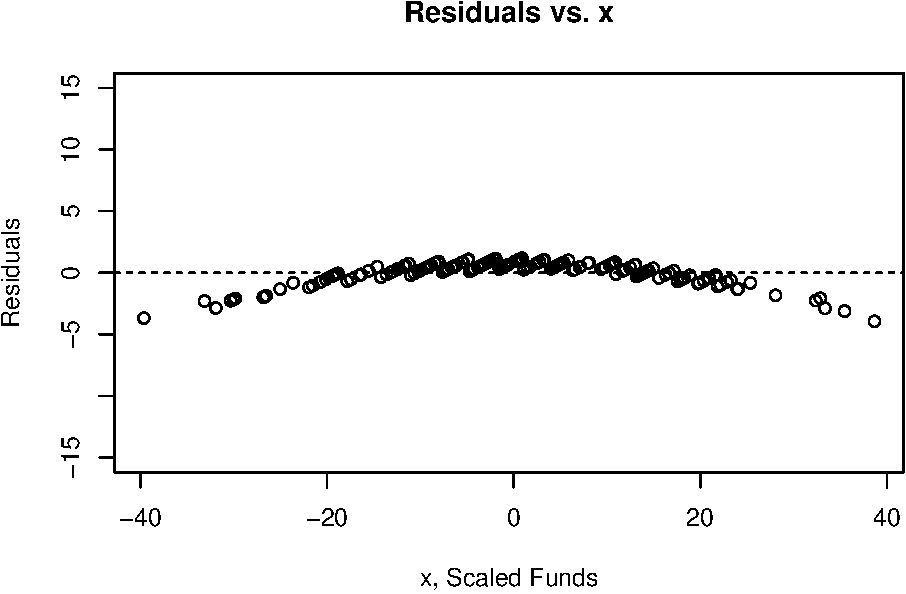
\includegraphics{Journal_files/figure-latex/unnamed-chunk-44-1.pdf}

\begin{Shaded}
\begin{Highlighting}[]
\FunctionTok{plot}\NormalTok{(reg.output, }\AttributeTok{which=}\DecValTok{3}\NormalTok{)}
\end{Highlighting}
\end{Shaded}

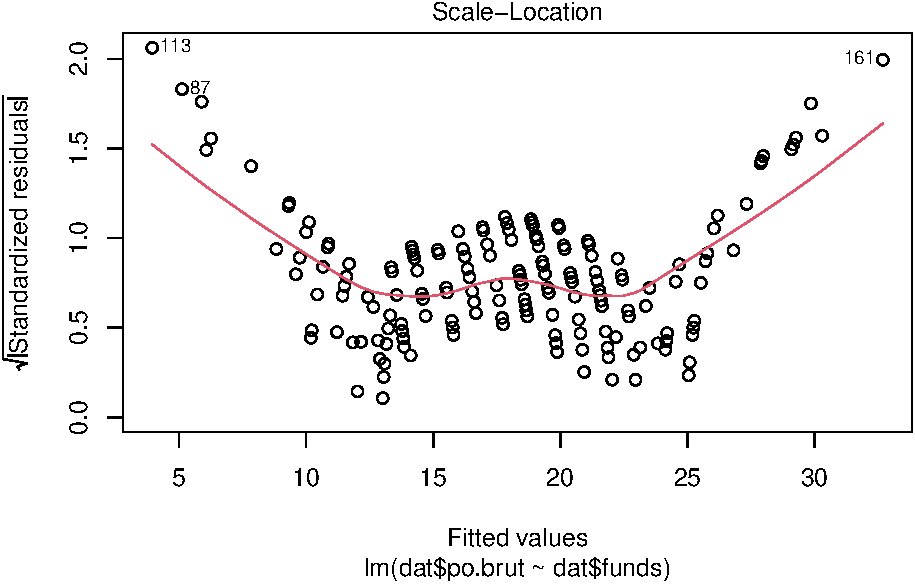
\includegraphics{Journal_files/figure-latex/unnamed-chunk-44-2.pdf}

\begin{Shaded}
\begin{Highlighting}[]
\FunctionTok{plot}\NormalTok{(reg.output, }\AttributeTok{which=}\DecValTok{2}\NormalTok{)}
\end{Highlighting}
\end{Shaded}

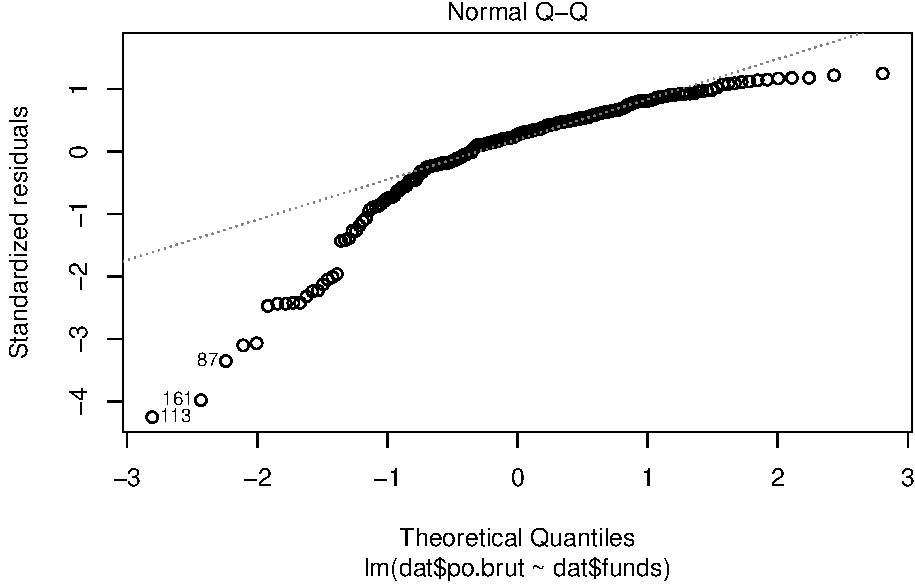
\includegraphics{Journal_files/figure-latex/unnamed-chunk-44-3.pdf}

Here, about three of the four assumptions seem to be satisfied.
Attempting to satisfy both the linearity and independence assumptions
with the residuals vs.~x plot, they seem to be satisfied in that the
majority of residuals seem to be centered around the dotted line,
however, the tails seem to be scaling down towards the bottom of the
graph, which may lead to discrepancies in independence, as there seems
to be a patterns. Attempting to satisfy the homoscedasticity assumption,
there seems to be a great discrepancy, and thus does not seem to be
satisfied. Here, there is a large pattern in the middle of the graph
which seems in the shape of a ``W'', where some residuals seem to have a
non-constant variance. With more time, I would attempt to transform the
graph to even out these residuals to try and create constant variance
and a graph without these outlier patterns. Lastly, the normal
population assumption seems to be satisfied, as the majority of the plot
falls within the dotted line (especially near the middle). However, once
again, the heavy tails of the graph seem the skew these quantities and
demonstrate some non-normally distributed values.

\emph{e. Answer the question of interest based on your analysis.}

Based on the analysis of these assumptions, it seems that my previous
response to the question holds proven, however with some discrepancies.
First, although the majority of the assumptions are proven, and thus the
null hypothesis could be rejected and my answer may hold, there are
still issues in non-constant variance and the tails of the graph dealing
with normal populations. Thus, the correlation should be taken as proven
along with the factors of some non-constant variance and population
outliers.

\hypertarget{problem-3-data-ethics-10-points}{%
\subsection{Problem 3: Data ethics (10
points)}\label{problem-3-data-ethics-10-points}}

\emph{Describe the dataset. Considering our lecture on data ethics, what
concerns do you have about the dataset? Once you perform your analysis
to answer the question of interest using this dataset, what concerns
might you have about the results?}

The dataset, again, considers the correlation in a singular year between
police department funding in millions in comparison to police brutality
incidents in each department. First, I believe there may be issues in
representativeness (regarding the non-constant variance and population
outliers discovered), bias in the sources and reporting of data (along
with its randomness), consent of victims of police brutality, and
testing for errors among certain user groups. With the results of the
dataset, some concerns might be that since this dataset only describes a
singular year correlating funding and brutality, it is not able to make
an assumption that may hold proven throughout time. Thus, this
correlation cannot be held proven past the year it was studied, and
doing so might heavily misrepresent the situation of correlation.
Additionally, the results should be more heavily fleshed out to get rid
of the non-constant variance and any other issues that might impede
interpretation. Thus, the correlation cannot describe past its year and
cannot be held proven without more exploration of the analysis.

\hypertarget{assignment-4}{%
\section{Assignment 4}\label{assignment-4}}

\hypertarget{page-1---chapter-3-data-visualization}{%
\subsection{Page 1 - Chapter 3: Data
Visualization}\label{page-1---chapter-3-data-visualization}}

install.packages(``tidyverse'', repos =
``\url{http://cran.us.r-project.org}'') \emph{Installing the package
`tidyverse'}

library(tidyverse) \emph{Scanning the library for the package
`tidyverse'}

mpg \emph{Loading the dataframe for a collection of variables dealing
with the car-related dataset, where ``displ'' is a car's engine size in
liters, and ``hwy'' is a car's fuel efficiency on the highway in miles
per gallon (mpg)}

ggplot(data = mpg) + geom\_point(mapping = aes(x = displ, y = hwy))
\emph{Creating a gg plot based on the ``mpg'' dataframe, showing
``displ'' on the x-axis and ``hwy'' on the y-axis}

ggplot(data = ) GEOM\_FUNCTION(mapping = aes()) \emph{Nonworking
graphing template for graphing with ggplot2}

ggplot(data = mpg) + geom\_point(mapping = aes(x = displ, y = hwy, color
= class)) \emph{Mapping the variables by color to reveal the class of
each car}

ggplot(data = mpg) + geom\_point(mapping = aes(x = displ, y = hwy, size
= class)) \emph{Warning because you should not map an unordered variable
(class) to an ordered aesthetic (size)}

ggplot(data = mpg) + geom\_point(mapping = aes(x = displ, y = hwy, alpha
= class)) \emph{Alpha controls transparency of points} ggplot(data =
mpg) + geom\_point(mapping = aes(x = displ, y = hwy, shape = class))
\emph{Shape controls the shape of points}

ggplot(data = mpg) + geom\_point(mapping = aes(x = displ, y = hwy),
color = ``blue'') \emph{Making all points in plot blue}

ggplot(data = mpg) + geom\_point(mapping = aes(x = displ, y = hwy, color
= ``blue'')) \emph{First Problem Encountered: parenthesis issue that
leaves color red}

ggplot(data = mpg) + geom\_point(mapping = aes(x = displ, y = hwy))
\emph{Second Problem Encountered: Should not be putting ``+''}

ggplot(data = mpg) + geom\_point(mapping = aes(x = displ, y = hwy)) +
facet\_wrap(\textasciitilde{} class, nrow = 2) \emph{Faceting plot by a
single variable}

ggplot(data = mpg) + geom\_point(mapping = aes(x = displ, y = hwy)) +
facet\_grid(drv \textasciitilde{} cyl) \emph{Faceting a plot on the
combination of two variables}

ggplot(data = mpg) + geom\_point(mapping = aes(x = drv, y = cyl))
\emph{Makes empty cells within the plot}

ggplot(data = mpg) + geom\_point(mapping = aes(x = displ, y = hwy)) +
facet\_grid(drv \textasciitilde{} .) ggplot(data = mpg) +
geom\_point(mapping = aes(x = displ, y = hwy)) + facet\_grid(.
\textasciitilde{} cyl) \emph{The ``.'' creates a unary function}

ggplot(data = mpg) + geom\_point(mapping = aes(x = displ, y = hwy)) +
facet\_wrap(\textasciitilde{} class, nrow = 2) \emph{This is the exact
same single-variable faceted plot as before}

ggplot(data = mpg) + geom\_point(mapping = aes(x = displ, y = hwy))
ggplot(data = mpg) + geom\_smooth(mapping = aes(x = displ, y = hwy))
\emph{Can change the geom (geometrical object used to represent data)
within a ggplot}

ggplot(data = mpg) + geom\_smooth(mapping = aes(x = displ, y = hwy,
linetype = drv)) \emph{Setting the linetype of a line}

ggplot(data = mpg) + geom\_smooth(mapping = aes(x = displ, y = hwy))
ggplot(data = mpg) + geom\_smooth(mapping = aes(x = displ, y = hwy,
group = drv)) ggplot(data = mpg) + geom\_smooth( mapping = aes(x =
displ, y = hwy, color = drv), show.legend = FALSE) \emph{Grouping data
for geoms when you map an aesthetic to a discrete variable}

ggplot(data = mpg) + geom\_point(mapping = aes(x = displ, y = hwy)) +
geom\_smooth(mapping = aes(x = displ, y = hwy)) \emph{Display multiple
geoms in the same plot}

ggplot(data = mpg, mapping = aes(x = displ, y = hwy)) + geom\_point() +
geom\_smooth() \emph{Passing a set of mappings to ggplot, treating them
as global mappings that apply to each geom in the graph}

ggplot(data = mpg, mapping = aes(x = displ, y = hwy)) +
geom\_point(mapping = aes(color = class)) + geom\_smooth()
\emph{Displaying different aesthetics in different layers to
extend/overwrite global mappings for that layer only}

ggplot(data = mpg, mapping = aes(x = displ, y = hwy)) +
geom\_point(mapping = aes(color = class)) + geom\_smooth(data =
filter(mpg, class == ``subcompact''), se = FALSE) \emph{Local data
argument in `geom\_smooth' overrudes that global data argument in ggplot
for that layer only}

ggplot(data = mpg, mapping = aes(x = displ, y = hwy, color = drv)) +
geom\_point() + geom\_smooth(se = FALSE) \emph{The data is not smoothed}

ggplot(data = mpg, mapping = aes(x = displ, y = hwy)) + geom\_point() +
geom\_smooth() ggplot() + geom\_point(data = mpg, mapping = aes(x =
displ, y = hwy)) + geom\_smooth(data = mpg, mapping = aes(x = displ, y =
hwy)) \emph{They are the same graphs because the aethetics were input
for all parts of the graph in both}

ggplot(data = diamonds) + geom\_bar(mapping = aes(x = cut)) \emph{ggplot
of the dataset ``diamonds''}

ggplot(data = diamonds) + stat\_count(mapping = aes(x = cut))
\emph{Recreating the last plot using ``stat\_count'' instead}

demo \textless- tribble( \textasciitilde cut, \textasciitilde freq,
``Fair'', 1610, ``Good'', 4906, ``Very Good'', 12082, ``Premium'',
13791, ``Ideal'', 21551 ) \emph{Bar chart where the height of the bar is
already present in the data}

ggplot(data = demo) + geom\_bar(mapping = aes(x = cut, y = freq), stat =
``identity'') \emph{Previous bar chart where the height of the bar is
generated by counting rows}

ggplot(data = diamonds) + geom\_bar(mapping = aes(x = cut, y =
stat(prop), group = 1)) \emph{Display a bar chart of proportion rather
than count}

ggplot(data = diamonds) + stat\_summary( mapping = aes(x = cut, y =
depth), fun.min = min, fun.max = max, fun = median ) \emph{Summarizes
the y values for each unique x value, drawing attention to the summary}

ggplot(data = diamonds) + geom\_bar(mapping = aes(x = cut, y =
after\_stat(prop))) ggplot(data = diamonds) + geom\_bar(mapping = aes(x
= cut, fill = color, y = after\_stat(prop))) \emph{A `group = 1' must be
added to make sure that the bar graphs are proportionate and accurately
portray the data}

ggplot(data = diamonds) + geom\_bar(mapping = aes(x = cut, color = cut))
ggplot(data = diamonds) + geom\_bar(mapping = aes(x = cut, fill = cut))
\emph{Coloring a barchart using either ``color'' or ``fill''}

ggplot(data = diamonds) + geom\_bar(mapping = aes(x = cut, fill =
clarity)) \emph{Filling the aesthetic with another variable, `clarity'}

ggplot(data = diamonds, mapping = aes(x = cut, fill = clarity)) +
geom\_bar(alpha = 1/5, position = ``identity'') ggplot(data = diamonds,
mapping = aes(x = cut, colour = clarity)) + geom\_bar(fill = NA,
position = ``identity'') \emph{To see the overlapping bars, need to make
the bars slightly transparent by setting `alpha' to a small value or
completely transparent by setting `fill=NA'}

ggplot(data = diamonds) + geom\_bar(mapping = aes(x = cut, fill =
clarity), position = ``fill'') \emph{Makes each set of stacked bars the
same height}

ggplot(data = diamonds) + geom\_bar(mapping = aes(x = cut, fill =
clarity), position = ``dodge'') \emph{Places overlapping objects
directly beside one another}

ggplot(data = mpg) + geom\_point(mapping = aes(x = displ, y = hwy),
position = ``jitter'') \emph{Avoiding gridding/overplotting by adding
`jitter,' adding random noise to the plot}

ggplot(data = mpg, mapping = aes(x = cty, y = hwy)) + geom\_point()
\emph{Problem that may be fixed with jittering}

ggplot(data = mpg, mapping = aes(x = class, y = hwy)) + geom\_boxplot()
ggplot(data = mpg, mapping = aes(x = class, y = hwy)) + geom\_boxplot()
+ coord\_flip() \emph{Switching the x and y axes}

nz \textless- map\_data(``nz'') ggplot(nz, aes(long, lat, group =
group)) + geom\_polygon(fill = ``white'', colour = ``black'') ggplot(nz,
aes(long, lat, group = group)) + geom\_polygon(fill = ``white'', colour
= ``black'') + coord\_quickmap() \emph{Sets aspect ratio correctly for
maps}

bar \textless- ggplot(data = diamonds) + geom\_bar( mapping = aes(x =
cut, fill = cut), show.legend = FALSE, width = 1 ) + theme(aspect.ratio
= 1) + labs(x = NULL, y = NULL) bar + coord\_flip() bar + coord\_polar()
\emph{Uses polar coordinates}

ggplot(data = mpg, mapping = aes(x = cty, y = hwy)) + geom\_point() +
geom\_abline() + coord\_fixed() \emph{Showing coordination between city
and highway mpg using fixed polar coordinates and reference lines}

ggplot(data = ) + ( mapping = aes(), stat = , position = ) + +
\emph{Nonworking graphic template for position adjustments, stats,
coordinate systems, and faceting}

\hypertarget{page-2---chapter-28-graphics-for-communication}{%
\subsection{Page 2 - Chapter 28: Graphics for
Communication}\label{page-2---chapter-28-graphics-for-communication}}

library(tidyverse) \emph{Scanning the library for the package
`tidyverse'}

ggplot(mpg, aes(displ, hwy)) + geom\_point(aes(color = class)) +
geom\_smooth(se = FALSE) + labs(title = ``Fuel efficiency generally
decreases with engine size'') \emph{Adding labels with `labs'}

ggplot(mpg, aes(displ, hwy)) + geom\_point(aes(color = class)) +
geom\_smooth(se = FALSE) + labs( title = ``Fuel efficiency generally
decreases with engine size'', subtitle = ``Two seaters (sports cars) are
an exception because of their light weight'', caption = ``Data from
fueleconomy.gov'' ) \emph{Adding more text to a graph using `subtitle'
and `caption'}

ggplot(mpg, aes(displ, hwy)) + geom\_point(aes(colour = class)) +
geom\_smooth(se = FALSE) + labs( x = ``Engine displacement (L)'', y =
``Highway fuel economy (mpg)'', colour = ``Car type'' ) \emph{Using
`labs' to replace the axis and legend titles}

df \textless- tibble( x = runif(10), y = runif(10) ) ggplot(df, aes(x,
y)) + geom\_point() + labs( x = quote(sum(x{[}i{]} \^{} 2, i == 1, n)),
y = quote(alpha + beta + frac(delta, theta)) ) \emph{Using mathematical
equations instead of text strings}

best\_in\_class \textless- mpg \%\textgreater\% group\_by(class)
\%\textgreater\% filter(row\_number(desc(hwy)) == 1) ggplot(mpg,
aes(displ, hwy)) + geom\_point(aes(colour = class)) +
geom\_text(aes(label = model), data = best\_in\_class) \emph{Using a
tibble to provide labels, pulling out the most efficient `car' in each
class with `dplyr' and then labeling it on the plot}

ggplot(mpg, aes(displ, hwy)) + geom\_point(aes(colour = class)) +
geom\_label(aes(label = model), data = best\_in\_class, nudge\_y = 2,
alpha = 0.5) \emph{`geom\_label' draws a rectangle behind the text and
`nudge\_y' parameter moves the labels above the corresponding points}

ggplot(mpg, aes(displ, hwy)) + geom\_point(aes(colour = class)) +
geom\_point(size = 3, shape = 1, data = best\_in\_class) +
ggrepel::geom\_label\_repel(aes(label = model), data = best\_in\_class)
\emph{The `ggrepel' pack automatically adjusts labels so they don't
overlap}

class\_avg \textless- mpg \%\textgreater\% group\_by(class)
\%\textgreater\% summarise( displ = median(displ), hwy = median(hwy) )
\#\textgreater{} \texttt{summarise()} ungrouping output (override with
\texttt{.groups} argument) ggplot(mpg, aes(displ, hwy, colour = class))
+ ggrepel::geom\_label\_repel(aes(label = class), data = class\_avg,
size = 6, label.size = 0, segment.color = NA ) + geom\_point() +
theme(legend.position = ``none'') \emph{Replacing the legends with
labels placed directly in the plot, also turning the legend off}

label \textless- mpg \%\textgreater\% summarise( displ = max(displ), hwy
= max(hwy), label = ``Increasing engine size is \nrelated to decreasing
fuel economy.'' ) ggplot(mpg, aes(displ, hwy)) + geom\_point() +
geom\_text(aes(label = label), data = label, vjust = ``top'', hjust =
``right'') \emph{Creating a new data frame to compute the maximum values
of x and y}

label \textless- tibble( displ = Inf, hwy = Inf, label = ``Increasing
engine size is \nrelated to decreasing fuel economy.'' ) ggplot(mpg,
aes(displ, hwy)) + geom\_point() + geom\_text(aes(label = label), data =
label, vjust = ``top'', hjust = ``right'') \emph{Using `Inf' to place
text on the borders of the plot, while using `tibble' to create the data
frame}

``Increasing engine size is related to decreasing fuel economy.''
\%\textgreater\% stringr::str\_wrap(width = 40) \%\textgreater\%
writeLines() \# Increasing engine size is related to decreasing fuel
economy. \emph{Automatically adding line breaks with the `stringr' line}

ggplot(mpg, aes(displ, hwy)) + geom\_point(aes(colour = class))
\emph{Part one of two, the input to create the following output:}

ggplot(mpg, aes(displ, hwy)) + geom\_point(aes(colour = class)) +
scale\_x\_continuous() + scale\_y\_continuous() +
scale\_colour\_discrete() \emph{Part two of two, the output where
ggplot2 automatically adds default scales}

ggplot(mpg, aes(displ, hwy)) + geom\_point() +
scale\_y\_continuous(breaks = seq(15, 40, by = 5)) \emph{Using `breaks'
to override the default choice of appearance of the ticks on the axes
and keys on the legend}

ggplot(mpg, aes(displ, hwy)) + geom\_point() +
scale\_x\_continuous(labels = NULL) + scale\_y\_continuous(labels =
NULL) \emph{Adding `NULL' to suppress the labels altogether}

presidential \%\textgreater\% mutate(id = 33 + row\_number())
\%\textgreater\% ggplot(aes(start, id)) + geom\_point() +
geom\_segment(aes(xend = end, yend = id)) + scale\_x\_date(NULL, breaks
= presidential\$start, date\_labels = ``'\%y'') \emph{Using a
presidential terms dataset, using `breaks' while working with few data
points to highlight exactly where the observations occur}

base \textless- ggplot(mpg, aes(displ, hwy)) + geom\_point(aes(colour =
class)) + base + theme(legend.position = ``left'') + base +
theme(legend.position = ``top'') + base + theme(legend.position =
``bottom'') + base + theme(legend.position = ``right'') \# the default
\emph{Using themes to control the non-data parts of the plot, where the
theme setting `legend.position' controls where the legend is drawn}

ggplot(mpg, aes(displ, hwy)) + geom\_point(aes(colour = class)) +
geom\_smooth(se = FALSE) + theme(legend.position = ``bottom'') +
guides(colour = guide\_legend(nrow = 1, override.aes = list(size = 4)))
\# \texttt{geom\_smooth()} using method = `loess' and formula `y
\textasciitilde{} x' \emph{Using `guides' to control the display of
individual legends, controlling the number of rows the legend uses with
`nrow,' and overriding one of the aesthetics to make the points bigger}

ggplot(diamonds, aes(carat, price)) + geom\_bin2d() ggplot(diamonds,
aes(log10(carat), log10(price))) + geom\_bin2d() \emph{Plotting
transformations of the variable to see a more precise relationship}

ggplot(diamonds, aes(carat, price)) + geom\_bin2d() + scale\_x\_log10()
+ scale\_y\_log10() \emph{Identical to the last plot except the axes are
labelled on the original data scale}

ggplot(mpg, aes(displ, hwy)) + geom\_point(aes(color = drv)) ggplot(mpg,
aes(displ, hwy)) + geom\_point(aes(color = drv)) +
scale\_colour\_brewer(palette = ``Set1'') \emph{Altering graphs to
create a color palette that may be distinguished even for those who are
color-blind}

ggplot(mpg, aes(displ, hwy)) + geom\_point(aes(color = drv, shape =
drv)) + scale\_colour\_brewer(palette = ``Set1'') \emph{Simpler
re-coloring techniques so that colored graphs can even be see in
black-and-white}

presidential \%\textgreater\% mutate(id = 33 + row\_number())
\%\textgreater\% ggplot(aes(start, id, colour = party)) + geom\_point()
+ geom\_segment(aes(xend = end, yend = id)) +
scale\_colour\_manual(values = c(Republican = ``red'', Democratic =
``blue'')) \emph{Using `scale\_colour\_manual' when you have a
predefined mapping between values and colors}

df \textless- tibble( x = rnorm(10000), y = rnorm(10000) ) ggplot(df,
aes(x, y)) + geom\_hex() + coord\_fixed() ggplot(df, aes(x, y)) +
geom\_hex() + viridis::scale\_fill\_viridis() + coord\_fixed()
\emph{Using the `viridis' package within `scale\_colour\_viridis' for a
continuous analog of the categorical ColorBrewer scales}

ggplot(df, aes(x, y)) + geom\_hex() + scale\_colour\_gradient(low =
``white'', high = ``red'') + coord\_fixed() \emph{Code does not override
the default scale}

ggplot(diamonds, aes(carat, price)) + geom\_point(aes(colour = cut),
alpha = 1/20) \emph{Difficulty on seeing the legend, must use
`override.aes' to make clearer}

ggplot(mpg, mapping = aes(displ, hwy)) + geom\_point(aes(color = class))
+ geom\_smooth() + coord\_cartesian(xlim = c(5, 7), ylim = c(10, 30))
mpg \%\textgreater\% filter(displ \textgreater= 5, displ \textless= 7,
hwy \textgreater= 10, hwy \textless= 30) \%\textgreater\%
ggplot(aes(displ, hwy)) + geom\_point(aes(color = class)) +
geom\_smooth() \emph{Using `coord\_cartesian' to zoom in on a region of
the plot}

suv \textless- mpg \%\textgreater\% filter(class == ``suv'') compact
\textless- mpg \%\textgreater\% filter(class == ``compact'') ggplot(suv,
aes(displ, hwy, colour = drv)) geom\_point() ggplot(compact, aes(displ,
hwy, colour = drv)) geom\_point() \emph{Expanding the limits of the
plots to match scales across the two plots}

x\_scale \textless- scale\_x\_continuous(limits =
range(mpg\(displ)) y_scale <- scale_y_continuous(limits = range(mpg\)hwy))
col\_scale \textless- scale\_colour\_discrete(limits = unique(mpg\$drv))
ggplot(suv, aes(displ, hwy, colour = drv)) geom\_point() x\_scale
y\_scale col\_scale ggplot(compact, aes(displ, hwy, colour = drv))
geom\_point() x\_scale y\_scale col\_scale \emph{Sharing scales across
multiple plots to train the scales with the limits of the full data}

ggplot(mpg, aes(displ, hwy)) geom\_point(aes(color = class))
geom\_smooth(se = FALSE) theme\_bw() \emph{Can customize the non-data
elements of the plot with a theme}

ggplot(mpg, aes(displ, hwy)) geom\_point() \emph{Sample code to save the
plots out of R in either `ggsave' or knitr}

ggsave(``my-plot.pdf'') \# Saving 7 x 4.33 in image \emph{Using `ggsave'
to save the image of the plots as a pdf}

\end{document}
